%%%%%%%%%%%%%%%%%%%%%%%%%%%%%%%%%%%%%%%%%%%%%%%%%%%%%%%%%%%%%%%%%%%%%%%%%%%%%%%%%%%%%%%%%%%%%
\chapter{Variety and stratification}

\section{Initial case: $\mathcal{F}$ and $\mathcal{F} \times \mathcal{F}$}\label{sec:inital_case}

We introduce the complete flag variety to give a bird's eye view on the whole section. Actually, the entire difficulty is bundled in this example.

\begin{setting}\label{set:initial_case}
Fix $n \geqslant 1$, we denote $\GL_n:=\GL_n(\mathbb{C})$, $B$, $T$, $N$, $W$ be the standard Borel subgroup, standard torus, unipotent subgroup, Weyl group respectively, i.e.,
{
\setlength\arraycolsep{1pt}
\renewcommand{\arraystretch}{0.6}
$$\GL_n= \begin{pmatrix}
* & \cdots & * \\[-1.4mm]
\vdots & \ddots & \vdots \\
* & \cdots & * 
\end{pmatrix} \quad
B= \begin{pmatrix}
* & \cdots & * \\[-1.4mm]
 & \ddots & \vdots \\
\scriptstyle 0 &  & * 
\end{pmatrix} \quad
T= \begin{pmatrix}
* &  & \scriptstyle 0 \\[-1.4mm]
 & \ddots &  \\
\scriptstyle 0 &  & * 
\end{pmatrix} \quad
N= \begin{pmatrix}
\scriptstyle 1 & \cdots & * \\[-1.4mm]
 & \ddots & \vdots \\
\scriptstyle 0 &  & \scriptstyle 1
\end{pmatrix} \quad
$$
$$W:= N_{\GL_n}(T)/T \cong S_n$$
}
\end{setting}

\subsection{$\mathcal{F}$}
\begin{defn}[Flag]
For a finite dimensional $\mathbb{C}$-vector space $V$, a flag of $V$ is an increasing sequence of subspaces of $V$:
$$F: 0 \subseteq M_1 \subseteq M_2 \subseteq \cdots \subseteq M_k = V.$$
$F$ is called a complete flag if $\dim V_j = j$ for all $j$, otherwise $F$ is called a partial flag.
\end{defn}

\begin{defn}[Complete flag variety]
The complete flag variety $\mathcal{F}$ is defined as 
\begin{equation*}
\begin{aligned}
  \mathcal{F}=\;& \GL_n/B \\ 
    \cong\;&  \left\{ \text{complete flags of } \mathbb{C}^n \right\} \\ 
      =\;& \left\{ 0 \subseteq M_1 \subseteq M_2 \subseteq \cdots \subseteq M_n = \mathbb{C}^n \;\middle|\; \dim M_j =j \right\} \\ 
       \cong\;&  \left\{ \text{Borel subgroups of } \GL_n \right\} \\
          =\;& \left\{ gBg^{-1} \;\middle|\; g \in \GL_n \right\} \\ 
\end{aligned}
\end{equation*}
\end{defn}

\begin{remark}\
\begin{enumerate}
\item $\mathcal{F}$ is a smooth projective variety of dimension $\frac{n(n+1)}{2}$, which can be seen from the embedding
$$\mathcal{F} \hookrightarrow \Gr(1,n) \times \cdots \times \Gr(n-1,n)$$

\item We implicitly give the base point of $\mathcal{F}$, which is not considered as the data of $\mathcal{F}$. Fix a standard basis of $\mathbb{C}^n$ by $\{v_1, \ldots, v_n \}$, we define the standard flag
$$F_{\Id}: 0 \subseteq \left< v_1 \right> \subseteq \left< v_1,v_2 \right> \subseteq \cdots \subseteq \left< v_1, \ldots, v_n \right> = \mathbb{C}^n.$$
\item We have the natural $\GL_n$-action on $\mathcal{F}$, which is considered as the data of $\mathcal{F}$.

For $g \in \GL_n$, we define the flag attached to $g$: 
$$F_g \triangleq gF_{\Id}: 0 \subseteq \left< gv_1 \right> \subseteq \left< gv_1,gv_2 \right> \subseteq \cdots \subseteq \left< gv_1, \ldots, gv_n \right> = \mathbb{C}^n.$$
Especially, for $w \in W=N_{\GL_n}(T)/T \cong S_n$, the flag attached to $w$
\begin{equation*}
\begin{aligned}
  F_w:\;&  0 \subseteq \left< \tilde{w}v_1 \right> \subseteq \left< \tilde{w}v_1,\tilde{w}v_2 \right> \subseteq \cdots \subseteq \left< \tilde{w}v_1, \ldots, \tilde{w}v_n \right> = \mathbb{C}^n\\ 
  &  0 \subseteq \left< v_{w(1)} \right> \subseteq \left< v_{w(1)},v_{w(2)} \right> \subseteq \cdots \subseteq \left< v_{w(1)}, \ldots, v_{w(n)} \right> = \mathbb{C}^n\\
\end{aligned}
\end{equation*}
does not depend on the choice of the lift $\tilde{w} \in N_{\GL_n}(T)$ of $w$.

Readers can verify that $\left\{ F_w \,\middle|\, w \in W \right\}$ are all $T$-fixed points of $\mathcal{F}$, while $\left\{ wBw^{-1} \,\middle|\, w \in W \right\}$ are all Borel subgroups of $G$ containing the standard torus $T$.
\item For $n=2$, $\mathcal{F} \cong \mathbb{P}^1$. We encourage readers to use $\mathbb{P}^1$ as a toy example for the whole theory.
\end{enumerate}
\end{remark}



\begin{table}[ht]
\centering
\begin{tabular}{|c|c|c|c|}
\hline
interpretation & $\GL_n/B$           & flags                       & Borel subgroups \\ \hline
base point     & $\Id$               & $F_{\Id}$                   & $B$             \\ \hline
$\GL_n$-action & left multiplication & $\{V_i\} \mapsto \{gV_i \}$ & conjugation     \\ \hline
general point  & $g$                 & $F_g$                       & $gBg^{-1}$      \\ \hline
\end{tabular}
\end{table}
        
$\mathcal{F}$ is a well-studied variety, and has many combinatorical properties. For example, from the well-known Bruhat decomposition, \footnote{For the most time the formula does not depend on the lift of $w$, so we abuse the notation of $w \in N_{\GL_n}(T)/T$ and $\tilde{w} \in N_{\GL_n}(T)$.}
$$\GL_n =\bigsqcup_{w\in W} BwB$$

We get a stratification of $\mathcal{F}$ by $B$-orbits:
$$\mathcal{F} = \GL_n/B \cong \bigsqcup_{w\in W} BwB/B$$
The $B$-orbit $BwB/B$ is called the \textbf{Schubert cell}, denoted by $\Omcell_w$. Since 
$$\Omcell_w=BwB/B \cong B/\left( B \cap wBw^{-1} \right) \cong \mathbb{A}^{l(w)},$$
the Schubert cell is an affine space of dimension $l(w)$.

As a result, we know a lot of information of $\mathcal{F}$:
%https://tex.stackexchange.com/questions/112576/math-mode-in-tabular-without-having-to-use-everywhere
\newcolumntype{C}{>{$}c<{$}} % math-mode version of "l" column type
\begin{table}[]
\centering
\begin{tabular}{|C|C|C|C|C|C|C|C|}
\hline
H^i(\mathcal{F}; \mathbb{C}) & 0 & 2 & 4 & 6  & 8  & 10 & 12 \\ \hline
1                            & 1 &   &   &    &    &    &    \\ \hline
2                            & 1 & 1 &   &    &    &    &    \\ \hline
3                            & 1 & 2 & 2 & 1  &    &    &    \\ \hline
4                            & 1 & 3 & 5 & 6  & 5  & 3  & 1  \\ \hline
5                            & 1 & 4 & 9 & 15 & 20 & 22 & 20 \\ \hline
\end{tabular}
\end{table}
\begin{table}[]
\centering
\begin{tabular}{C|C|C}
\hline
G    & \text{Orbit}                       & G\text{-fixed points}  \\ \hline
GL_n & \mathcal{F} \cong \GL_n/B          & \varnothing            \\ \hline
B    & \Omcell_w \cong B/(B \cap wBw^{-1}) & \{F_{\Id} \}           \\ \hline
T    & -                                  & \{F_w |  \, w \in W \} \\ \hline
\end{tabular}
\end{table}

$\overline{\Omcell}_w \subseteq \mathcal{F}$ is called the \textbf{Schubert variety}. It is well-known that
$$\overline{\Omcell}_w= \bigsqcup_{w' \leq w} \Omcell_w$$
as a set. Especially, for any $s\in W$ with $l(s)=1$, denote $P_s=B \sqcup BsB$,
$$\overline{\Omcell}_s= \Omcell_{\Id} \sqcup \Omcell_s = B/B \sqcup BsB/B = P_s/B \cong \mathbb{P}^1.$$
For other Schubert variety, the structures are quite dedicate and far away from the scope of this master thesis. For example, most  Schubert varieties are not smooth.


\subsection{$\mathcal{F} \times \mathcal{F}$}\label{subsec:product_of_F}
As a more complicated geometrical object, $\mathcal{F} \times \mathcal{F}$ works as the base space for the Steinberg variety, which turns out to be the central focus in the thesis. $\mathcal{F} \times \mathcal{F}$ has naturally a diagonal $\GL_n$-action:
$$\GL_n \times \mathcal{F} \times \mathcal{F} \longrightarrow \mathcal{F} \times \mathcal{F} \qquad (g,F_1,F_2) \longmapsto (gF_1,gF_2).$$
Under this action, $\mathcal{F} \times \mathcal{F}$ has a stratification consisting of $GL_n$-orbits, indexed by the Weyl group:
$$\GL_n \setminus (\mathcal{F} \times \mathcal{F}) \cong \GL_n \setminus (\GL_n/B \times \GL_n/B) \cong B \setminus \GL_n /B \cong W \quad \text{ as sets.}$$

Denote $\OOmcell_{w'}:= \GL_n \cdot (F_{\Id}, F_{w'})$, then $\mathcal{F} \times \mathcal{F}= \sqcup_{w'} \OOmcell_{w'}$. Moreover, by the orbit-stabilizer theorem, we get
$$\OOmcell_{w'} \cong \GL_n/\left( B \cap w'B(w')^{-1}  \right)$$
which is an $\mathbb{A}^{l(w')}$-bundle over $\mathcal{F}$, as shown below:
% https://q.uiver.app/?q=WzAsMyxbMCwwLCJcXG1hdGhiYntBfV57bCh3Jyl9IFxcY29uZyBCL1xcbGVmdCggQiBcXGNhcCB3J0IodycpXnstMX0gIFxccmlnaHQpIl0sWzEsMCwiXFxHTF9uL1xcbGVmdCggQiBcXGNhcCB3J0IodycpXnstMX0gIFxccmlnaHQpIl0sWzEsMSwiXFxtYXRoY2Fse0Z9PVxcR0xfbi9CXFxoc3BhY2V7NW1tfSJdLFswLDFdLFsxLDJdXQ==
\[\begin{tikzcd}
	{\mathbb{A}^{l(w')} \cong B/\left( B \cap w'B(w')^{-1}  \right)} & {\GL_n/\left( B \cap w'B(w')^{-1}  \right)} \\
	& {\hspace{-10mm}\mathcal{F}=\GL_n/B}
	\arrow[from=1-1, to=1-2]
	\arrow[from=1-2, to=2-2]
\end{tikzcd}\]

Different from $\mathcal{F}$, the $\GL_n$-action on $\mathcal{F} \times \mathcal{F}$ is not transitive. To facilitate the stratification of $\mathcal{F}\times \mathcal{F}$, we introduce the twisted $\GL_n \times \GL_n$-action:
$$\GL_n \times \GL_n \times \mathcal{F} \times \mathcal{F} \longrightarrow \mathcal{F} \times \mathcal{F} \qquad (g_1,g_2,F_g,F_{g'}) \longmapsto (F_{g_1g},F_{g_1(gg_2g^{-1}) g'}).$$
If we write $\underline{F}_{g,g'}:= (F_g,F_{gg'}) \in \mathcal{F} \times \mathcal{F}$, then 
$$(g_1,g_2) \cdot\underline{F}_{g,g'}=\underline{F}_{g_1g,g_2g'}.$$

This $\GL_n \times \GL_n$-action is now transitive, and decompose $\mathcal{F}\times \mathcal{F}$ as disjoint union of finite many $B \times B$-orbits, which are compatible with $G$-orbits:

\begin{equation*}
\begin{aligned}
  &\OOmcell_{w,w'}:=\; (B \times B) \cdot \underline{F}_{w,w'} \subseteq \mathcal{F}\times \mathcal{F}\\ 
  &\mathcal{F}\times \mathcal{F}= \bigsqcup_{w, w'\in W} \OOmcell_{w,w'} \qquad\OOmcell_{w'}= \bigsqcup_{w\in W} \OOmcell_{w,w'} \\
\end{aligned}
\end{equation*}
\begin{equation}\label{eq:twisted_stabilizer}
\begin{aligned}
   \OOmcell_{w,w'} \cong\;& (B \times B)/\left\{ (g_1,g_2) \in B \times B  \;\middle|\; (g_1,g_2) \cdot (F_w,F_{ww'})=(F_w,F_{ww'})  \right\}\\
=\;& (B \times B)/\left\{ (g_1,g_2) \in B \times B  \;\middle|\; g_1wB=wB, g_1wg_2w'B=ww'B  \right\}\\   
=\;& (B \times B)/\left\{ (g_1,g_2) \in B \times B  \;\middle|\; g_1wB=wB, (w^{-1}g_1w)g_2w'B=w'B  \right\}\\   
=\;& (B \times B)/\left\{ (g_1,g_2) \in B \times B  \;\middle|\; g_1\in wBw^{-1}, g_2 \in (w^{-1}g_1^{-1}w) \left(w'Bw'^{-1}\right)  \right\}\\  
=\;& (B \times B)/\left\{ (g_1,g_2) \in \left(B \cap wBw^{-1}\right) \times (w^{-1}g_1^{-1}w)  \left(B \cap  w'Bw'^{-1}\right)    \right\}\\  
   \cong\;& B/(B \cap wBw^{-1}) \times B/(B \cap w'Bw'^{-1}) \cong \mathbb{A}^{l(w)+l(w')}
\end{aligned}
\end{equation}
We conclude the information of orbits and fixed points of $\mathcal{F}\times \mathcal{F}$ in Table \ref{table:orbit_of_F*F}:

\begin{table}[ht]
\centering
\[
\begin{array}{c|c|c}
\hline
G                  & \text{Orbit}              & G\text{-fixed points}                      \\ \hline
\GL_n \times \GL_n & \mathcal{F} \times \mathcal{F} & \varnothing                                \\ \hline
\GL_n              & \OOmcell_{w'}              & \varnothing                                \\ \hline
B \times B         & \OOmcell_{w,w'}            & \{F_{\Id,\Id} \}                           \\ \hline
T                  & -                         & \{\underline{F}_{w,w'} |  \, w,w' \in W \} \\ \hline
\end{array}
\]
\caption{Orbit and fixed points of $\mathcal{F}\times \mathcal{F}$}
\label{table:orbit_of_F*F}
\end{table}

Like $\mathcal{F}$, we also study the closure of $\OOmcell_{w'}$ and $\OOmcell_{w,w'}$ in special case. It can be shown that 
$$\overline{\OOmcell}_{w'} = \bigsqcup_{x'\leq w'} \OOmcell_{x'} \qquad 
\overline{\OOmcell}_{w,w'} = \bigsqcup_{x \leq w, x'\leq w'} \OOmcell_{x,x'}$$
as a set. Especially, for any $s \in W$ with $l(s)=1$, \footnote{Here, $\GL_n \times^B X$ is called contracted product. Roughly, it is defined by
$$\GL_n \times^B X :=\GL_n \times X/\big( (gb,x) \sim (g,bx) \big)$$
We will discuss contracted product in Subsection \ref{subsec:contracted_product} thoroughly.}

\begin{equation*}
\begin{aligned}
 \overline{\OOmcell}_{s} = \OOmcell_{\Id}\sqcup \OOmcell_{s} \cong\;& 
  \GL_n /(B \cap sBs^{-1}) &&\sqcup \GL_n/B \\ 
  \cong\;&  \GL_n \times^{B} \left(B/(B \cap sBs^{-1})\right)\hspace{-0.4cm} &&\sqcup \GL_n \times^{B} (B/B) \\ 
  \cong\;& \GL_n \times^{B} (BsB/B) &&\sqcup \GL_n \times^{B} (B/B)  \\ 
  \cong\;& \GL_n \times^{B} (P_s/B)&& \\ 
\end{aligned}
\end{equation*}
is an $\mathcal{F}$-bundle over $\mathbb{P}^1$. Also, 
\begin{equation*}
\begin{aligned}
\overline{\OOmcell}_{\Id,s} = \OOmcell_{\Id,s} \sqcup \OOmcell_{\Id,\Id} \cong\;& 
 \big(B/B \times BsB/B\big) \sqcup \big(B/B \times B/B\big)  \\ 
 \cong\;& P_s/B \cong \mathbb{P}^1
\end{aligned}
\end{equation*}
Other closure can be highly singular.

\begin{eg}
In the table, $n=3$, $t=(12)$, $s=(23)$. In this case, $\mathcal{F}\times \mathcal{F}$ has $6$ $\GL_3$-orbits, and each $\GL_3$-orbits decompose as $6$ $B\times B$-orbits, with dimensions equal to $l(w)+l(w')$.
\begin{table}[ht]
  \vspace{0cm}
    \centering  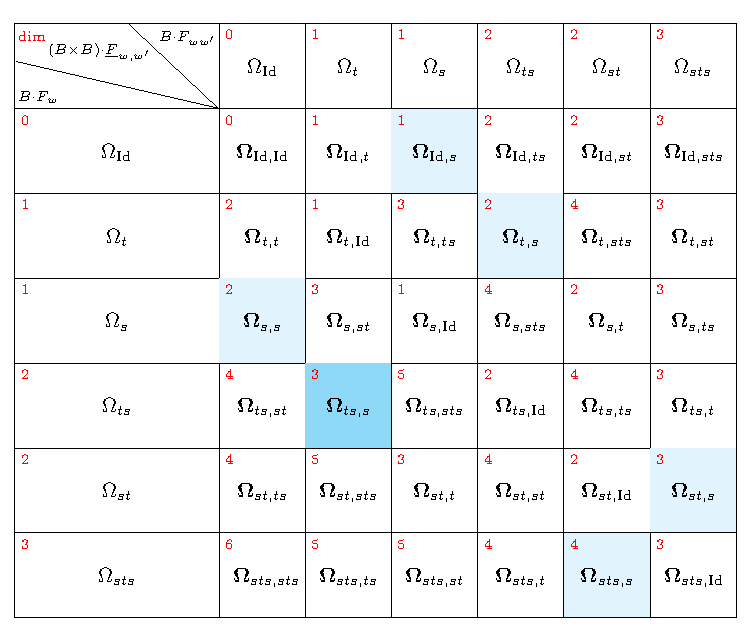
\includegraphics[width=12.8cm]{figures/table/table_1.pdf}
      \label{fig:stratifications_of_FF}
        \caption{stratifications of $\mathcal{F}\times \mathcal{F}$}
        
\end{table}

We can also see the $\GL_3$-orbit (and its closure) from the table, for example,
\begin{equation*}
\begin{aligned}
  \OOmcell_{s}=\;& \OOmcell_{\Id,s} \sqcup
  \OOmcell_{t,s} \sqcup
  \OOmcell_{s,s} \sqcup
  \OOmcell_{ts,s} \sqcup
  \OOmcell_{st,s} \sqcup
  \OOmcell_{sts,s}  \\ 
  \overline{\OOmcell}_{s}=\;& \OOmcell_{s} \sqcup \OOmcell_{\Id} = \bigsqcup_{w} (\OOmcell_{w,s} \sqcup \OOmcell_{w,\Id})
\end{aligned}
\end{equation*}
\end{eg}



Now wee understand a lot about $\mathcal{F}$ and $\mathcal{F} \times \mathcal{F}$, and the whole process of analysis(investigations?) will be applied repeatedly in Section \ref{sec:typical_variety} and \ref{sec:stratification}. 
\section{Quiver}
To introduce more complicated spaces and discuss their stratifications, we fix notations related to quiver and algebraic group in the following sections.

Roughly speaking, a quiver is a directed multigraph permitting loops.

\begin{defn}[Quiver]
A quiver is a quadruple 
$$Q=(Q_0,Q_1,s,t)$$
where
\begin{itemize}[noitemsep,topsep=0pt]
\item $Q_0$ is a non-empty set consisting of vertices of $Q$,
\item $Q_1$ is a set consisting of arrows of $Q$,
\item $s:Q_1 \longrightarrow Q_0$ is a map indicating the start vertex of arrows,
\item $t:Q_1 \longrightarrow Q_0$ is a map indicating the terminal vertex of arrows.
\end{itemize}
\end{defn}

\begin{remark}\label{rmk:quiver_restriction}
In the first part of our master thesis, all the quivers are supposed to be connected and finite (i.e., $Q_0$, $Q_1$ are finite sets). We will only encounter disconnected and infinite quiver as Auslander--Reiten quiver later on.
\end{remark}

\begin{eg}
The following graphs are quivers.

\begin{table}[ht]
\centering
\begin{tabular}{@{\extracolsep{5mm}}ccc}
$$\begin{tikzcd}[ampersand replacement=\&]
	\bullet \& \bullet \& \bullet \& \bullet
	\arrow[from=1-1, to=1-2]
	\arrow[from=1-3, to=1-2]
	\arrow[from=1-4, to=1-3]
\end{tikzcd}$$ & $$\begin{tikzcd}[ampersand replacement=\&]
 	\bullet \arrow[out=120,in=60,loop,looseness=8]
 	\arrow[out=0,in=-60,loop,looseness=8]
 	\arrow[out=-120,in=-180,loop,looseness=8]
 \end{tikzcd}$$ & $$\begin{tikzcd}[ampersand replacement=\&]
 	1 \& 2
 	\arrow["a", curve={height=-6pt}, from=1-1, to=1-2]
 	\arrow["b"', curve={height=6pt}, from=1-1, to=1-2]
 \end{tikzcd}$$ \\
 quiver of type $A_3$ & $3$-loop quiver $L(3)$ & $2$-Kronecker quiver $K(2)$
\end{tabular}
\vspace{5mm}
\end{table}
The reader can easily read the quadruple of quivers from the graphs. Take $Q=K(2)$ as an example, we have 
$$Q_0=\{1,2\}, \qquad Q_1=\{a,b\} \qquad s,t: \{a,b\}\longrightarrow \{1,2\}$$
by $s(a)=s(b)=1$, $t(a)=t(b)=2$.

For convenience, we mainly use simpler quivers as examples:

\begin{table}[ht]
\centering
\begin{tabular}{@{\extracolsep{5mm}}ccc}
$$\begin{tikzcd}[ampersand replacement=\&]
	\bullet 
\end{tikzcd}$$ & $$\begin{tikzcd}[ampersand replacement=\&]
	\bullet \& \bullet 
	\arrow[from=1-1, to=1-2]
 \end{tikzcd}$$ & $$\begin{tikzcd}[ampersand replacement=\&]
 	\bullet \arrow[out=30,in=-30,loop,looseness=6]
 \end{tikzcd}$$ \\
 trivial quiver & quiver of type $A_1$ & $1$-loop quiver $L(1)$
\end{tabular}
\vspace{5mm}
\end{table}

\end{eg}

From those quivers we are able to construct relatively complicated algebraic and geometrical objects.

\begin{defn}[Quiver representation]
Fix a quiver $Q$. A representation of $Q$ consists of the following data:
\begin{itemize}[noitemsep,topsep=0pt]
\item A finite dimensional $\mathbb{C}$-vector space $V_i$ for each vertex $i \in Q_0$;
\item A $\mathbb{C}$-linear map $V_a: V_{s(a)} \longrightarrow V_{t(a)}$ for each arrow $a \in Q_1$.
\end{itemize}
\end{defn}
\begin{eg}
A representation of $1$-loop quiver $L(1)$ is a $2$-tuple
$$(V, \; \alpha: V \longrightarrow V)$$
which is equivalent to a (finite dimensional) $\mathbb{C}[t]$-module.
\end{eg}
\begin{remark}
The equivalence appeared in the example can actually be generalized to arbitrary quivers. For a quiver $Q$, we can define the path algebra $\mathbb{C}Q$, and view any $Q$-representation as $\mathbb{C}Q$-module, and vice versa.
\end{remark}

For many constructions, we only care about the data of vector space.
\begin{defn}[$Q$-vector space/Vector space with quiver partition]
Fix a quiver $Q$, a $Q$-vector space is a finite dimensional $\mathbb{C}$-vector space with the direct sum decomposition
$$V= \bigoplus_{i \in Q_0} V_i.$$
The dimension vector of a $Q$-vector space is defined as
$$\dimv V =\left( \dim_{\mathbb{C}} V_i \right)_{i \in Q_0} \subseteq \prod_{i \in Q_0} \mathbb{Z}.$$
\end{defn} 

On the country, given $\dimvec{d} \in \prod_{i \in Q_0} \mathbb{N}_{\geqslant 0}$, we can construct a canonical $Q$-vector space of dimension vector $\dimvec{d}$, as follows:
$$V= \bigoplus_{i \in Q_0} V_i \qquad \text{ with } V_i= \mathbb{C}^{\dimvec{d}_i}.$$

\begin{defn}
The total dimension vector of a $Q$-vector space $V$ is defined as
$$\left| \dimv V  \right|:=\dim_{\mathbb{C}} V.$$
For $\dimvec{d} \in \prod_{i \in Q_0} \mathbb{N}_{\geqslant 0}$, denote $\abdimvec{d}:= \sum_{i \in Q_0} \dimvec{d}_i$.
\end{defn}
\begin{defn}[Space of representations with given dimension vector]
For any quiver $Q$, dimension vector $\dimvec{d}$, fix the canonical $Q$-vector space $V= \bigoplus_{i \in Q_0} V_i$, the space of representations with dimension vector $\dimvec{d}$ is defined as
\begin{equation*}
\begin{aligned}
  \Rep_{\dimvec{d}}(Q)=\;&  \left\{ (V_i,V_a: V_{s(a)} \longrightarrow V_{t(a)} ) \text{ as a representation of $Q$}  \right\} \\ 
  =\;& \bigoplus_{a \in Q_1} \Hom \left(\mathbb{C}^{\dimvec{d}_{s(a)}},\mathbb{C}^{\dimvec{d}_{t(a)}}\right)
\end{aligned}
\end{equation*}

Since we encode the information of vector space in $\dimvec{d}$, $\Rep_{\dimvec{d}}(Q)$ only records the information of linear maps.
\end{defn}

For both $Q$-vector space and $Q$-representations, we can define (complete) flags.

\begin{defn}[Flag with quiver] \label{def:flag_with_quiver}
For a quiver representation $V \in \rep(Q)$, a flag of $V$ is defined as an increasing sequence of subrepresentation of $V$, i.e.,
$$F: 0 \subseteq M_1 \subseteq \ldots \subseteq M_k=V \qquad M_j\in \rep(Q). $$
For a $Q$-vector space $V=\oplus_{i \in Q_0}V_i$, a (quiver-graded) flag of $V$ is defined as an increasing sequence of $Q$-subspace of $V$, i.e.,
$$F: 0 \subseteq M_1 \subseteq \ldots \subseteq M_k=V \qquad M_j=\bigoplus_{i \in Q_0}M_{j,i}. $$
For both $Q$-vector space and $Q$-representation, $F$ is called a complete flag if $k=\dim_{\mathbb{C}} V$ and
$$\dim_{\mathbb{C}} M_j=j \qquad \text{ for any }j \in \{1,\ldots, \abdimvec{d}  \}$$
\end{defn}
For the flag we also have the notation of dimension vector.
\begin{defn}[flag-type dimension vector]
For any flag $F: 0 \subseteq M_1 \subseteq \ldots \subseteq M_k=V$, the dimension vector of $F$ is defined as
$$\ftdimvec{d}=\big(\!\dimv M_j   \big)_{j \in \{1,\ldots,k\}} \subseteq \prod_{\substack{i \in Q_0 \\ j \in \{1,\ldots,k\}}} \mathbb{Z}.$$
$\ftdimvec{d}$ is called a flag-type dimension vector if $\ftdimvec{d}$ is the dimension vector of some complete flag $F$, i.e., \footnote{For convenience, we denote $M_0$ by 0.}
$$\left| \dimv M_{j+1}/M_j \right|=1 \qquad \text{ for any }j \in \{0,\ldots, \abdimvec{d}-1  \}.$$
\end{defn}

\begin{eg}\label{eg:5-case-0}
For quiver $Q: i \longrightarrow i'$, $\dimvec{d}=(3,2)$, the canonical $Q$-vector space of dimension vector $\dimvec{d}$ is
\begin{equation*}
\begin{aligned}
  V=\;& V_i \oplus V_{i'} \\ 
  =\;& \left< v_1,v_2,v_3 \right>_{\mathbb{C}} \oplus \left< v_4,v_5 \right>_{\mathbb{C}}\\ 
\end{aligned}
\end{equation*}
The flag 
$$F: 0 \subseteq \left< v_4 \right>
\subseteq \left< v_4,v_1 \right>
\subseteq \left< v_4,v_1,v_2 \right>
\subseteq \left< v_4,v_1,v_2,v_5 \right>
\subseteq \left< v_4,v_1,v_2,v_5,v_3 \right>=V$$
is a complete flag of $V$, with dimension vector
{
\def\arraystretch{0.8}
$$\ftdimvec{d}= \begin{pmatrix}
3,2\\ 2,2 \\ 2,1 \\ 1,1 \\ 0,1
\end{pmatrix}.$$
}
\end{eg}
\begin{remark}
The flag-type dimension vector $\ftdimvec{d}$ can be viewed as a partition on set $\{1,\ldots, \abdimvec{d} \}$, i.e., a map
$$\ptt: \{1,\ldots, \abdimvec{d}  \} \longrightarrow Q_0$$
such that $\#\ptt^{-1}(i)=\dimvec{d}_i$.\footnote{The partition corresponding to $\ptt$ is$$\{1,\ldots, \abdimvec{d}\}=\bigsqcup_{i \in Q_0}\ptt^{-1}(i).$$} . As an example,
{
\def\arraystretch{0.8}
$$\ftdimvec{d}= \begin{pmatrix}
3,2\\ 2,2 \\ 2,1 \\ 1,1 \\ 0,1
\end{pmatrix} \quad\text{ corresponds to }\quad \{1,2,3,4,5\}= \{2,3,5\} \sqcup \{1,4\}.$$
}
\end{remark}

\section{Symmetric group calculus}

As a reminder, we recall some basic diagrams referring to the elements in $S_n$, and do some calculations by these diagrams. We will also relate cosets with flag-type dimension vectors.

Fix a quiver $Q$ and dimension vector $\dimvec{d}$. Later (Definition \ref{def:absalggp}, \ref{def:relalggp}) we will define 
$$\absgp{W}_{\abdimvec{d}}= S_{\abdimvec{d}} \qquad W_{\dimvec{d}} = \prod_{i \in Q_0} S_{\dimvec{d}_i} \leqslant \absgp{W}_{\abdimvec{d}}$$
For simplicity, we take $Q_0=\{1,\ldots, k\}$, then $W_{\dimvec{d}}= S_{\dimvec{d}_1} \times \cdots \times S_{\dimvec{d}_k}$ embed in  $S_{\abdimvec{d}}$ in the most natural way.

\begin{remark}
We have different ways to express $\ww \in \absgp{W}_{\abdimvec{d}}= S_{\abdimvec{d}}$. For example, take $\abdimvec{d}=5$, $\ww \in S_5$ by
$$\ww(1)=4,\quad \ww(2)=3,\quad \ww(3)=1,\quad \ww(4)=5,\quad \ww(5)=2,$$ 
then
{
\setlength\arraycolsep{1pt}
\renewcommand{\arraystretch}{0.6}
\begin{equation*}
\begin{aligned}
  \ww=\;& (14523)= \begin{pmatrix}
  1\,2\,3\,4\,5\\ 4\,3\,1\,5\,2
  \end{pmatrix} = \parbox[h][][c]{3cm}{\permutation[tkzpic=1]{4,3,1,5,2}}\hspace{-2mm} =\begin{bmatrix}
  &&\scriptstyle 1&&\\
  &&&&\scriptstyle 1\\
  &\scriptstyle 1&&&\\
  \scriptstyle 1&&&&\\
  &&&\scriptstyle 1&
  \end{bmatrix} \\ 
  =\;& (23)(34)(45)(12)(23)(12) = \hspace{0mm} 
  \parbox[h][][c]{3cm}{ \begin{tikzpicture}
   \permutation[
   height=0.2,
   bullb=0,
   floor=5,
   tkzpic=0,
   type=1
   ]{2,1,3,4,5}
   \permutation[
   height=0.2,
   bulla=0,
   bullb=0,
   floor=4,
   tkzpic=0,
   type=0
   ]{1,3,2,4,5}
   \permutation[
   height=0.2,
   bulla=0,
   bullb=0,
   floor=3,
   tkzpic=0,
   type=0
   ]{2,1,3,4,5}
    \permutation[
    height=0.2,
    bulla=0,
    bullb=0,
    floor=2,
    tkzpic=0,
    type=0
    ]{1,2,3,5,4}
   \permutation[
   height=0.2,
   bulla=0,
   bullb=0,
   floor=1,
   tkzpic=0,
   type=0
   ]{1,2,4,3,5}
   \permutation[
   height=0.2,
   bulla=0,
   floor=0,
   tkzpic=0,
   type=-1
   ]{1,3,2,4,5}
   \end{tikzpicture}}
\end{aligned}
\end{equation*}
}

Even though all expressions give us the same amount of information, the diagram presents them more vividly. For example, each intersection of strands corresponds to a simple reflection, so we read from the diagram that $l(\ww)=6$. Readers can also check that
\begin{equation*}
\begin{aligned}
  &  l(\ww s_1)=5,\quad l(\ww s_2)=5,\quad l(\ww s_3)=7,\quad l(\ww s_4)=5,\\ 
  &  l(s_1\ww)=7,\quad l(s_2\ww)=5,\quad l(s_3\ww)=5,\quad l(s_4\ww)=7,\\ 
\end{aligned}
\end{equation*} 
where $s_i:=(i,i+1) \in S_5$ are simple reflections.

\end{remark}

\begin{defn}[Special elements in the Weyl group]
For $i \in \left\{ 1, \ldots , \abdimvec{d}-1 \right\}$, the simple reflection is defined as
$$s_i:=(i,i+1) \in  S_{\abdimvec{d}}.$$
We denote
\begin{equation*}
\begin{aligned}
  \Pi=\;&  \Big\{ s_i \in S_{\abdimvec{d}} \;\Big|\; i \in \left\{ 1, \ldots , \abdimvec{d}-1 \right\} \Big\} \\ 
    \Pi_{\dimvec{d}}=\;&  \Big\{ s_i \in S_{\dimvec{d}_1} \times \cdots \times S_{\dimvec{d}_k} \;\Big|\; i \in \left\{ 1, \ldots , \abdimvec{d}-1 \right\} \Big\} \\ 
    =\;&\left\{ s_1,\ldots, s_{\abdimvec{d}-1} \right\} \smallsetminus \left\{s_{\dimvec{d}_1},s_{\dimvec{d}_1+\dimvec{d}_2},\ldots,s_{\dimvec{d}_1+\cdots+\dimvec{d}_{k-1}} \right\} \\
\end{aligned}
\end{equation*}
to be the set of simple reflections in $\absgp{W}_{\abdimvec{d}}$ and $W_{\dimvec{d}}$, respectively.

We also denote $\ww_{\max} \in \absgp{W}_{\abdimvec{d}}$, $w_{\max} \in W_{\dimvec{d}}$ to be the longest elements in $\absgp{W}_{\abdimvec{d}}$, $W_{\dimvec{d}}$, respectively.
\end{defn}

We discuss about right cosets $W_{\dimvec{d}}\setminus\absgp{W}_{\abdimvec{d}}$ and minimal length coset representatives now.

Multiplying on left by $w\in W_{\dimvec{d}}$ is equivalent to plugging in a diagram representing $w \in W_{\dimvec{d}}$ underneath the original diagram. Therefore, we connect some bottom points by lines, indicating that switching them will cause no trouble. Furthermore, we color different parts to make the following fact more explicitly.

\begin{fact}
Every element $\ww_{\max} \in W_{\dimvec{d}}\setminus\absgp{W}_{\abdimvec{d}}$ corresponds to a partition on set $\left\{ 1, \ldots , \abdimvec{d} \right\}$ (of a given number partition $\dimvec{d}$), which corresponds to a flag-type dimension vector $\ftdimvec{d}$.
\end{fact}

\begin{eg}\label{eg:3-case-0.1}
\begin{equation*}
\begin{aligned}
\parbox[h][][c]{3cm}{
 \begin{tikzpicture}
 \vpartition[
 floor=0,
 tkzpic=0,
 type=0
 ]{{5}}
 \tie[color=red,bull=1,bulletie=0.04,style=solid,tieheight=0]{{1},{2},{3}}
 \tie[color=red,bull=1,bulletie=0.04,style=solid]{{3,1},{1,0}}
 \tie[color=red,bull=1,bulletie=0.04,style=solid]{{5,1},{2,0}}
 \tie[color=red,bull=1,bulletie=0.04,style=solid]{{2,1},{3,0}}
 \tie[color=blue,bull=1,bulletie=0.04,style=solid]{{1,1},{4,0},{5,0},{4,1}}
 \end{tikzpicture}
 }
  =\hspace{8mm}& 
\parbox[h][][c]{3cm}{
 \begin{tikzpicture}
 \vpartition[
 floor=0,
 tkzpic=0,
 type=0
 ]{{5}}
 \tie[color=red,bull=1,bulletie=0.04,style=solid,tieheight=0]{{1},{2},{3}}
 \tie[color=red,bull=1,bulletie=0.04,style=solid]{{2,1},{1,0}}
 \tie[color=red,bull=1,bulletie=0.04,style=solid]{{3,1},{2,0}}
 \tie[color=red,bull=1,bulletie=0.04,style=solid]{{5,1},{3,0}}
 \tie[color=blue,bull=1,bulletie=0.04,style=solid]{{1,1},{4,0},{5,0},{4,1}}
 \end{tikzpicture}
 } \qquad   \text{ in } \Wd\setminus \WWd \\
 since\hspace{5.7cm}&\hspace{10cm}\\
%\shortintertext{since}
\parbox[h][][c]{3cm}{
 \begin{tikzpicture}
 \vpartition[
 floor=0,
 tkzpic=0,
 type=0
 ]{{5}}
 \tie[color=red,bull=1,bulletie=0.04,style=solid,tieheight=0]{{1},{2},{3}}
 \tie[color=red,bull=1,bulletie=0.04,style=solid]{{2,2},{3,1},{1,0}}
 \tie[color=red,bull=1,bulletie=0.04,style=solid]{{3,2},{1,1},{2,0}}
 \tie[color=red,bull=1,bulletie=0.04,style=solid]{{5,2},{2,1},{3,0}}
 \tie[color=blue,bull=1,bulletie=0.04,style=solid]{{1,2},{4,1},{4,0}}
 \tie[color=blue,bull=1,bulletie=0.04,style=solid]{{4,2},{5,1},{5,0}}
 \tie[color=red,bull=1,bulletie=0.04,style=solid]{{1,1},{2,1},{3,1}} 
 \tie[color=red,bull=1,bulletie=0.04,style=solid]{{1,0},{2,0},{3,0}} 
 \tie[color=blue,bull=1,bulletie=0.04,style=solid]{{4,1},{5,1}}
 \tie[color=blue,bull=1,bulletie=0.04,style=solid]{{4,0},{5,0}}
 \end{tikzpicture}
 }
  =\hspace{8mm}& 
\parbox[h][][c]{3cm}{
 \begin{tikzpicture}
% \vpartition[
% floor=1,
% tkzpic=0,
% type=0
% ]{{5}}
 \tie[color=red,bull=1,bulletie=0.04,style=solid,tieheight=0]{{1},{2},{3}}
 \tie[color=red,bull=1,bulletie=0.04,style=solid]{{2,2},{1,0}}
 \tie[color=red,bull=1,bulletie=0.04,style=solid]{{3,2},{2,0}}
 \tie[color=red,bull=1,bulletie=0.04,style=solid]{{5,2},{3,0}}
 \tie[color=blue,bull=1,bulletie=0.04,style=solid]{{1,2},{4,0},{5,0},{4,2}} 
 \end{tikzpicture}
 } \qquad   \text{ in } \WWd \\
 \end{aligned}
 \end{equation*}

This coset corresponds to the partition $\{1,2,3,4,5 \}= \{2,3,5\} \sqcup \{1,4\}$.

\end{eg}

It is easy to see from the diagram that in every coset, there exists an unique element $u \in \absgp{W}_{\abdimvec{d}}$ of minimal length. We collect these minimal length coset representatives as a set, and denote it by $\MinWd$.\footnote{In some references $\MinWd$ is also denoted by $\Shuffled$, since those elements can be thought as ways off riffle shuffling several words together.}

\begin{proposition}
For any $\ww \in \absgp{W}_{\abdimvec{d}}$, exists unique $w \in \Wd$, $u \in \MinWd$ such that $\ww=wu$. 
\end{proposition}
\begin{ex}
For $u \in \MinWd$, $s_i \in \Pi$, show that
\begin{equation*}
\begin{aligned}
us_iu^{-1}\in W_{\dimvec{d}} \quad\Longrightarrow&\quad us_iu^{-1}=s_{u(i)} \in \Pi_{\dimvec{d}},\\
us_iu^{-1}\notin W_{\dimvec{d}} \quad\Longrightarrow&\quad us_i \in \MinWd.
\end{aligned}
\end{equation*}
An example is shown in Table \ref{table:Lie_alg}.
\end{ex}

We finish this section with figures and examples.
% https://q.uiver.app/?q=WzAsOSxbMywwLCJcXE1pbldkIl0sWzMsMSwiV197XFxkaW12ZWN7ZH19XFxzZXRtaW51c1xcYWJzZ3B7V31fe1xcYWJkaW12ZWN7ZH19Il0sWzIsMSwiXFxhYnNncHtXfV97XFxhYmRpbXZlY3tkfX0iXSxbNCwxLCIwIl0sWzEsMSwiV197XFxkaW12ZWN7ZH19Il0sWzAsMSwiMCJdLFs2LDAsInUiXSxbNSwxLCJcXHd3PXd1Il0sWzYsMSwiXFxmdGRpbXZlY3tkfSJdLFswLDEsIlxcY29uZyJdLFswLDIsIiIsMix7InN0eWxlIjp7InRhaWwiOnsibmFtZSI6Imhvb2siLCJzaWRlIjoiYm90dG9tIn19fV0sWzIsMV0sWzEsM10sWzQsMl0sWzUsNF0sWzcsOCwiIiwwLHsic3R5bGUiOnsidGFpbCI6eyJuYW1lIjoibWFwcyB0byJ9fX1dLFs2LDgsIiIsMix7InN0eWxlIjp7InRhaWwiOnsibmFtZSI6Im1hcHMgdG8ifX19XV0=
\[\begin{tikzcd}
	&&& \MinWd &&& u \\
	0 & {W_{\dimvec{d}}} & {\absgp{W}_{\abdimvec{d}}} & {W_{\dimvec{d}}\setminus\absgp{W}_{\abdimvec{d}}} & 0 & {\ww=wu} & {\ftdimvec{d}}
	\arrow["\cong", from=1-4, to=2-4]
	\arrow[hook', from=1-4, to=2-3]
	\arrow[from=2-3, to=2-4]
	\arrow[from=2-4, to=2-5]
	\arrow[from=2-2, to=2-3]
	\arrow[from=2-1, to=2-2]
	\arrow[maps to, from=2-6, to=2-7]
	\arrow[maps to, from=1-7, to=2-7]
\end{tikzcd}\]

\begin{eg}\label{eg:5-case-1}
In this table, $\abdimvec{d}=5$, $\dimvec{d}=(3,2)$, typical elements would be
$$\ww = \parbox[h][][c]{3cm}{\permutation[tkzpic=1,type=0]{4,3,1,5,2}} \quad
w =\parbox[h][][c]{3cm}{\permutation[tkzpic=1,type=0]{3,1,2,5,4}} \quad
u =\parbox[h][][c]{3cm}{
 \begin{tikzpicture}
 \vpartition[
 floor=0,
 tkzpic=0,
 type=0
 ]{{5}}
 \tie[color=red,bull=1,bulletie=0.04,style=solid,tieheight=0]{{1},{2},{3}}
 \tie[color=red,bull=1,bulletie=0.04,style=solid]{{2,1},{1,0}}
 \tie[color=red,bull=1,bulletie=0.04,style=solid]{{3,1},{2,0}}
 \tie[color=red,bull=1,bulletie=0.04,style=solid]{{5,1},{3,0}}
 \tie[color=blue,bull=1,bulletie=0.04,style=solid]{{1,1},{4,0},{5,0},{4,1}}
 
 \end{tikzpicture}
 } \quad  $$
 {
 
 %https://tex.stackexchange.com/questions/394775/vertical-space-distribution-when-arraystretch-is-increased
\def\arraystretch{2}
 \begin{table}[ht]
 $$
 \begin{array}{l|l|r|c}
 \hline
 \multicolumn{1}{c|}{\text{set}} & \multicolumn{1}{c|}{\text{element}} & \multicolumn{1}{c|}{\text{special element}} & \text{others} \\ \hline
\absgp{W}_{\abdimvec{d}} = S_5 & \ww,x                               &   \ww_{\max}=  \lbox{\parbox[h][][c]{1.5cm}{\permutation[tkzpic=1,type=0,scale=0.5]{5,4,3,2,1}}  }                                      &   \Pi_{\phantom{d}}=\{s_1,s_2,s_3,s_4 \}            \\ \hline
W_{\dimvec{d}} = S_3 \times S_2      & w                                   &     w_{\max}= \lbox{\parbox[h][][c]{1.5cm}{\permutation[tkzpic=1,type=0,scale=0.5]{3,2,1,5,4}}    }                                    &  \Pi_{\dimvec{d}}=\{s_1,s_2,\phantom{s_3,}s_4 \}              \\ \hline
W_{\dimvec{d}}\setminus\absgp{W}_{\abdimvec{d}} \cong (S_3 \times S_2) \setminus S_5 & \ww, \ftdimvec{d}                   &          \parbox[h][][c]{1.6cm}{\parbox[h][][c]{1.5cm}{ \begin{tikzpicture}[scale=0.5]
 \vpartition[
 floor=0,
 tkzpic=0,
 type=0
 ]{{5}}
 \tie[color=red,bull=1,bulletie=0.04,style=solid,tieheight=0]{{1},{2},{3}}
 \tie[color=red,bull=1,bulletie=0.04,style=solid]{{3,1},{1,0}}
 \tie[color=red,bull=1,bulletie=0.04,style=solid]{{5,1},{2,0}}
 \tie[color=red,bull=1,bulletie=0.04,style=solid]{{2,1},{3,0}}
 \tie[color=blue,bull=1,bulletie=0.04,style=solid]{{1,1},{4,0},{5,0},{4,1}}
 \end{tikzpicture}} }                                   &    \Compd           \\ \hline
\MinWd =\left\{\parbox[h][][c]{1.5cm}{ \begin{tikzpicture}[scale=0.5]
 \vpartition[
 floor=0,
 tkzpic=0,
 type=0
 ]{{5}}
 \tie[color=red,bull=1,bulletie=0.04,style=solid,tieheight=0]{{1},{2},{3}}
 \tie[color=red,bull=1,bulletie=0.04,style=solid]{{2,1},{1,0}}
 \tie[color=red,bull=1,bulletie=0.04,style=solid]{{3,1},{2,0}}
 \tie[color=red,bull=1,bulletie=0.04,style=solid]{{5,1},{3,0}}
 \tie[color=blue,bull=1,bulletie=0.04,style=solid]{{1,1},{4,0},{5,0},{4,1}}
 \end{tikzpicture}}  ,\ldots \right\}  & u                                   &                                       \parbox[h][][c]{1.5cm}{ \begin{tikzpicture}[scale=0.5]
 \vpartition[
 floor=0,
 tkzpic=0,
 type=0
 ]{{5}}
 \tie[color=red,bull=1,bulletie=0.04,style=solid,tieheight=0]{{1},{2},{3}}
 \tie[color=red,bull=1,bulletie=0.04,style=solid]{{2,1},{1,0}}
 \tie[color=red,bull=1,bulletie=0.04,style=solid]{{3,1},{2,0}}
 \tie[color=red,bull=1,bulletie=0.04,style=solid]{{5,1},{3,0}}
 \tie[color=blue,bull=1,bulletie=0.04,style=solid]{{1,1},{4,0},{5,0},{4,1}}
 \end{tikzpicture}}      &   \Shuffled            \\ \hline
 \end{array}
 $$
 \end{table}
 }
 %调整表格。。。大难题
\end{eg}

\begin{eg}\label{eg:3-case-1}
In this table, 
$$\abdimvec{d}=3,\quad \dimvec{d}=(1,2),\qquad \WWd=S_3,\quad \Wd=S_1 \times S_2,\qquad s=(12),\quad t=(23).$$ The columns "order of basis" and "Borel subgroups" will be introduced in Definition \ref{def:special_flags} and Remark \ref{rmk:Borel_difference}.

\begin{table}[ht]
  \vspace{0cm}
    \centering  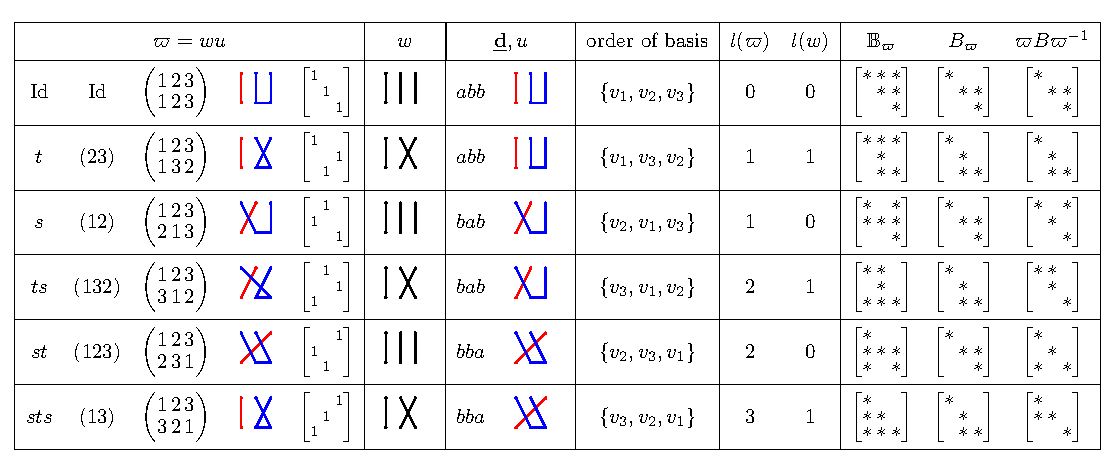
\includegraphics[width=15cm]{figures/table/table_basic_information.pdf}
      \caption{basic information of $(1,2)$-case}  
      \label{table:smalleg_Weyl}     
        \end{table}
        
\end{eg}
\section{Algebraic group and Lie algebra}
In this section we fix notations of algebraic group and Lie algebras. Later, the algebraic group will act on varieties, and some Lie algebra will serve as tangent spaces.



\begin{setting}\label{set:Qvs}
We fix a quiver $Q$, a dimension vector $\dimvec{d}$ and a $Q$-vector space 
$$V=\bigoplus_{i \in Q_0} V_i \qquad \text{with } V_i=\mathbb{C}^{\dimvec{d}_i}.$$
When a basis of $V$ is needed, we fix a total order on $Q_0$, and denote
$$V=\left< v_1, \ldots v_{\abdimvec{d}} \right> $$
where
$$V_i=\left< v_{f_i+1}, \ldots v_{f_i+\dimvec{d}_i} \right> \qquad f_i= \sum_{i' < i} \dimvec{d}_{i'}.$$
\end{setting}

\subsection{Algebraic group}

\begin{defn}[absolute algebraic groups]\label{def:absalggp}
%The following algebraic groups are not related to the quiver partition of $V$.
We set
$$\absgp{G}_{\abdimvec{d}}:= \GL(V)=\GL_{\abdimvec{d}}(\mathbb{C}),$$
and $\absgp{B}_{\abdimvec{d}}$, $\absgp{T}_{\abdimvec{d}}$, $\absgp{N}_{\abdimvec{d}}$ are corresponding standard Borel, torus and unipotent subgroups.

The Weyl group is
$$\absgp{W}_{\abdimvec{d}}:= N_{\absgp{G}_{\abdimvec{d}}}(\absgp{T}_{\abdimvec{d}})/\absgp{T}_{\abdimvec{d}} \cong S_{\abdimvec{d}}.$$

For $\ww \in \absgp{W}_{\abdimvec{d}}$, we define\footnote{As usual, we abuse the notation of $\ww$ and its lift.}
$$\absgp{B}_{\ww}:= \ww \absgp{B}_{\abdimvec{d}} \ww^{-1}.$$
We will view $\absgp{B}_{\ww}$ as the stabilizer of the flag $F_{\ww}$ with $\absgp{G}_{\abdimvec{d}}$-action.
\end{defn}

We also have a series of algebraic groups compatible with the quiver partition of $V$, and they're more common in this thesis.

\begin{defn}[relative algebraic groups]\label{def:relalggp}

We set
$$G_{\dimvec{d}}:= \bigoplus_{i \in Q_0}\GL(V_i)=\GL_{\dimvec{d}_i}(\mathbb{C}) \subseteq \absgp{G}_{\abdimvec{d}},$$
and $B_{\dimvec{d}}$, $T_{\dimvec{d}}$, $N_{\dimvec{d}}$ are corresponding standard Borel, torus and unipotent subgroups.

The Weyl group is
$$W_{\dimvec{d}}:= N_{G_{\dimvec{d}}}(T_{\dimvec{d}})/T_{\dimvec{d}} \cong \prod_{i \in Q_0}S_{\dimvec{d}_i}.$$

For $\ww=wu \in W_{\dimvec{d}}$, we define
$$B_{\ww}:= w B_{\dimvec{d}} w^{-1}.$$
We will view $B_{\ww}$ as the stabilizer of the flag $F_{\ww}$ with $G_{\dimvec{d}}$-action.
\end{defn}

\begin{remark}\label{rmk:Borel_difference}
Be careful that $B_{\ww} \neq \ww B_{\dimvec{d}} \ww^{-1}$. Actually,
$$B_{\ww}= \ww \absgp{B}_{\abdimvec{d}}\ww^{-1} \cap B_{\dimvec{d}}=wB_{\dimvec{d}}w^{-1}$$
The difference is clearly shown in Table \ref{table:smalleg_Weyl}.
\end{remark}

We also have a series of algebraic groups with subscription as elements in the Weyl group:
\begin{defn}[more algebraic groups]
For $\ww, \ww'' \in \absgp{W}_{\abdimvec{d}}$, define
\begin{equation*}
\begin{aligned}
  N_{\ww}:=\;& R_u(B_{\ww}),  \\ 
  N_{\ww,\ww''}:=\;& N_{\ww} \cap N_{\ww''},  \\ 
  M_{\ww,\ww''}:=\;& N_{\ww}/N_{\ww,\ww''},  \\ 
\end{aligned}
\end{equation*}
where $R_u$ denotes for the unipotent radical.

For $s \in \Pi$ such that $\ww s \ww^{-1} \in W_d$ (i.e., $W_{\dimvec{d}}\ww=W_{\dimvec{d}}\ww s$), define
\begin{equation*}
\begin{aligned}
  P_{\ww,\ww s}:\xlongequal{\ww =wu}\;& w\left( B_{\dimvec{d}} usu^{-1} B_{\dimvec{d}} \cup B_{\dimvec{d}} \right)w^{-1} \\ 
  \xlongequal{\phantom{\ww =wu}}\;&  B_{\ww} \ww s\ww^{-1} B_{\ww} \cup B_{\ww}  \\ 
\end{aligned}
\end{equation*}
\end{defn}
\begin{remark}
One can easily show that $N_{\ww, \ww s}=R_u (P_{\ww, \ww s})$.
\end{remark}
%problems on making short vertical space
%https://tex.stackexchange.com/questions/183562/how-to-reduce-vertical-space-in-matrix?newreg=ca78ba434426423a8be8ce4f1df4548c
%https://tex.stackexchange.com/questions/643384/horizontal-spacing-bmatrix-in-align-environment
%https://tex.stackexchange.com/questions/275725/adjusting-separation-between-matrix-entries
{\setlength\arraycolsep{1pt}
\renewcommand{\arraystretch}{0.6}

%small fonts: use \scriptstyle instead of \scriptsize

%vertical line:
%https://tex.stackexchange.com/questions/33519/vertical-line-in-matrix-using-latexit

\makeatletter
\renewcommand*\env@matrix[1][*\c@MaxMatrixCols c]{%
  \hskip -\arraycolsep
  \let\@ifnextchar\new@ifnextchar
  \array{#1}}
\makeatother
\begin{eg}[Follows Example \ref{eg:5-case-1}] \label{eg:5-case-2}
For $\abdimvec{d}=5$, $\dimvec{d}=(3,2)$, $\ww =\hspace{-3mm} \parbox[h][][c]{2cm}{\permutation[tkzpic=1,type=0,scale=0.5]{4,3,1,5,2}}$\hspace{-7mm}, 
$w =\hspace{-3mm}\parbox[h][][c]{2cm}{\permutation[tkzpic=1,type=0,scale=0.5]{3,1,2,5,4}}$\hspace{-7mm}, $s=s_2$, we compute all the algebraic groups we mentioned:
\begin{equation*}
\begin{aligned}
  &\absgp{G}_{\abdimvec{d}}= \begin{pmatrix}
  * & * & * & * & * \\
  * & * & * & * & * \\
  * & * & * & * & * \\
  * & * & * & * & * \\
  * & * & * & * & * \\
  \end{pmatrix}&
  \absgp{B}_{\abdimvec{d}}=
  \begin{pmatrix}
  * & * & * & * & * \\
   & * & * & * & * \\
   &  & * & * & * \\
   &  &  & * & * \\
   &  &  &  & * \\
  \end{pmatrix}&&
  \absgp{T}_{\abdimvec{d}}=
  \begin{pmatrix}
  * &  &  &  &  \\
   & * &  &  &  \\
   &  & * &  &  \\
   &  &  & * &  \\
   &  &  &  & * \\
  \end{pmatrix}&&
  \absgp{N}_{\abdimvec{d}}=
  \begin{pmatrix}
  \scriptstyle 1 & * & * & * & * \\
   & \scriptstyle 1 & * & * & * \\
   &  & \scriptstyle 1 & * & * \\
   &  &  & \scriptstyle 1 & * \\
   &  &  &  & \scriptstyle 1 \\
  \end{pmatrix}
    \\
  &\absgp{W}_{\abdimvec{d}}\cong S_5&
  \absgp{B}_{\ww}=
   \begin{pmatrix}
  * & * &  &  & * \\
   & * &  &  &  \\
  * & * & * &  & * \\
  * & * & * & * & * \\
   & * &  &  & * \\
  \end{pmatrix}&&
  \absgp{B}_{\ww s}=
     \begin{pmatrix}
    * & * & *  &  & * \\
     & * &  &  &  \\
     & * & * &  & * \\
    * & * & * & * & * \\
     & * &  &  & * \\
    \end{pmatrix}&&
  \\
  &G_{\dimvec{d}}\;=
  \begin{pmatrix}[ccc|cc]
  * & * & * &  &  \\
  * & * & * &  &  \\
  * & * & * &  &  \\
     \hline
   &  &  & * & * \\ 
   &  &  & * & * \\ 
  \end{pmatrix}&
  B_{\dimvec{d}}=
    \begin{pmatrix}[ccc|cc]
    * & * & * &  &  \\
     & * & * &  &  \\
     &  & * &  &  \\
        \hline
     &  &  & * & * \\ 
     &  &  &  & * \\ 
    \end{pmatrix}&&
  T_{\dimvec{d}}=
    \begin{pmatrix}[ccc|cc]
     * &  &  &  &  \\
       & * &  &  &  \\
       &  & * &  &  \\
          \hline
       &  &  & * &  \\
       &  &  &  & * \\
    \end{pmatrix}&&
  N_{\dimvec{d}}=
         \begin{pmatrix}[ccc|cc]
          \scriptstyle 1 & * & * &  &  \\
           & \scriptstyle 1 & * &  &  \\
           &  & \scriptstyle 1 &  &  \\
              \hline
           &  &  & \scriptstyle 1 & * \\ 
           &  &  &  & \scriptstyle 1 \\ 
          \end{pmatrix}  
  \\
&W_{\dimvec{d}}\cong S_3 \times S_2&
  B_{\ww}=
   \begin{pmatrix}[ccc|cc]
  * & * &  &  &  \\
   & * &  &  &  \\
  * & * & * &  &  \\
     \hline
   &  &  & * &  \\
   &  &  & * & * \\
  \end{pmatrix}&&
  B_{\ww s}=
     \begin{pmatrix}[ccc|cc]
  * &  &  &  &  \\
  * & * &  &  &  \\
  * & * & * &  &  \\
     \hline
   &  &  & * &  \\
   &  &  & * & * \\
    \end{pmatrix}&&
  \\
   &N_{\ww}=
    \begin{pmatrix}[ccc|cc]
   \scriptstyle 1 & * &  &  &  \\
    & \scriptstyle 1 &  &  &  \\
   * & * & \scriptstyle 1 &  &  \\
      \hline
    &  &  & \scriptstyle 1 &  \\
    &  &  & * & \scriptstyle 1 \\
   \end{pmatrix}&
   N_{\ww,\ww s}=
      \begin{pmatrix}[ccc|cc]
   \scriptstyle 1 &  &  &  &  \\
    & \scriptstyle 1 &  &  &  \\
   * & * & \scriptstyle 1 &  &  \\
      \hline
    &  &  & \scriptstyle 1 &  \\
    &  &  & * & \scriptstyle 1 \\
     \end{pmatrix}&& 
   M_{\ww,\ww s}=
      \begin{pmatrix}[ccc|cc]
   \scriptstyle 1 & * &  &  &  \\
    & \scriptstyle 1 &  &  &  \\
   \scriptstyle- & \scriptstyle- & \scriptstyle 1 &  &  \\
      \hline
    &  &  & \scriptstyle 1 &  \\
    &  &  & \scriptstyle- & \scriptstyle 1 \\
     \end{pmatrix}&& 
   P_{\ww,\ww s}=
      \begin{pmatrix}[ccc|cc]
   * & * &  &  &  \\
   * & * &  &  &  \\
   * & * & * &  &  \\
   \hline
    &  &  & * &  \\
    &  &  & * & * \\
     \end{pmatrix}
\end{aligned}
\end{equation*}




\end{eg}
}
\subsection{Lie algebra}
For the Lie algebra, we use the corresponding Fraktur-font symbols:
\begin{equation*}
\begin{aligned}
  & \boldsymbol{\mathfrak{g}}_{\abdimvec{d}}, &&\boldsymbol{\mathfrak{b}}_{\abdimvec{d}}, &&\boldsymbol{\mathfrak{t}}_{\abdimvec{d}}, &&\boldsymbol{\mathfrak{n}}_{\abdimvec{d}}, &&\boldsymbol{\mathfrak{b}}_{\ww}  \\
  & \mathfrak{g}_{\dimvec{d}},
  &&\mathfrak{b}_{\dimvec{d}},
  &&\mathfrak{t}_{\dimvec{d}},
  &&\mathfrak{n}_{\dimvec{d}},
  &&\mathfrak{b}_{\ww},\\
  & \mathfrak{n}_{\ww},\hspace{5mm}
  &&\mathfrak{n}_{\ww,\ww''},
  &&\mathfrak{m}_{\ww,\ww''},
  &&\mathfrak{p}_{\ww,\ww s},
  &&\\
\end{aligned}
\end{equation*}

We also have to encode the information of representations as Lie algebra. Notice that
$$\Hom (V_{s(a)},V_{t(a)}) \hookrightarrow \Hom(V,V) \cong \boldsymbol{\mathfrak{g}}_{\abdimvec{d}} \qquad f \longmapsto \iota_{t(a)} \circ f \circ \pi_{s(a)}$$
realizes $\Hom (V_{s(a)},V_{t(a)})$ as a Lie subalgebra of $\boldsymbol{\mathfrak{g}}_{\abdimvec{d}}$, so 
$$  \Rep_{\dimvec{d}}(Q)= \bigoplus_{a \in Q_1} \Hom \left(\mathbb{C}^{\dimvec{d}_{s(a)}},\mathbb{C}^{\dimvec{d}_{t(a)}}\right) \subseteq \bigoplus_{a \in Q_1} \boldsymbol{\mathfrak{g}}_{\abdimvec{d}}.$$
\begin{defn}[Lie algebras connected with representations]
For $\ww \in \absgp{W}_{\abdimvec{d}}$, denote temperately 
$$V_{\ww,j}:= \left< e_{\ww(1)},\ldots e_{\ww(j)} \right> \subseteq V.$$
We define Lie subalgebras of $\Rep_{\dimvec{d}}(Q)$ as follows.
%https://tex.stackexchange.com/questions/352752/align-inside-left-right

$$\mathfrak{r}_{\ww}:=\; \left\{ (f_a)_{a\in Q_1} \in \Rep_{\dimvec{d}}(Q) \;\middle| \;  f_a(V_{\ww,j} \cap V_{s(a)}) \subseteq V_{\ww,j} \text{ for any } j \right\},$$
\begin{equation*}
\begin{aligned}
  \mathfrak{r}_{\ww,\ww''}:=\;& \mathfrak{r}_{\ww} \cap \mathfrak{r}_{\ww''},  \\ 
  \mathfrak{d}_{\ww,\ww''}:=\;& \mathfrak{r}_{\ww}/\mathfrak{r}_{\ww,\ww''},  \\ 
\end{aligned}
\end{equation*}

\end{defn}
\begin{eg}[Follows Example \ref{eg:5-case-2}]\label{eg:5-case-3}
Consider the quiver $\begin{tikzcd}[ampersand replacement=\&]
	\textcolor{red}{\bullet} \& \textcolor{blue}{\bullet} 
	\arrow[from=1-1, to=1-2]
 \end{tikzcd}$, and $u =\parbox[h][][c]{2cm}{
  \begin{tikzpicture}[scale=0.5]
  \vpartition[
  floor=0,
  tkzpic=0,
  type=0
  ]{{5}}
  \tie[color=red,bull=1,bulletie=0.04,style=solid,tieheight=0]{{1},{2},{3}}
  \tie[color=red,bull=1,bulletie=0.04,style=solid]{{2,1},{1,0}}
  \tie[color=red,bull=1,bulletie=0.04,style=solid]{{3,1},{2,0}}
  \tie[color=red,bull=1,bulletie=0.04,style=solid]{{5,1},{3,0}}
  \tie[color=blue,bull=1,bulletie=0.04,style=solid]{{1,1},{4,0},{5,0},{4,1}}
  
  \end{tikzpicture}
  }$\hspace{-7mm}. Table \ref{table:Lie_alg} gives us an example of the shape of these Lie algebras. 
\begin{table}[ht]
  \vspace{0cm}
    \centering  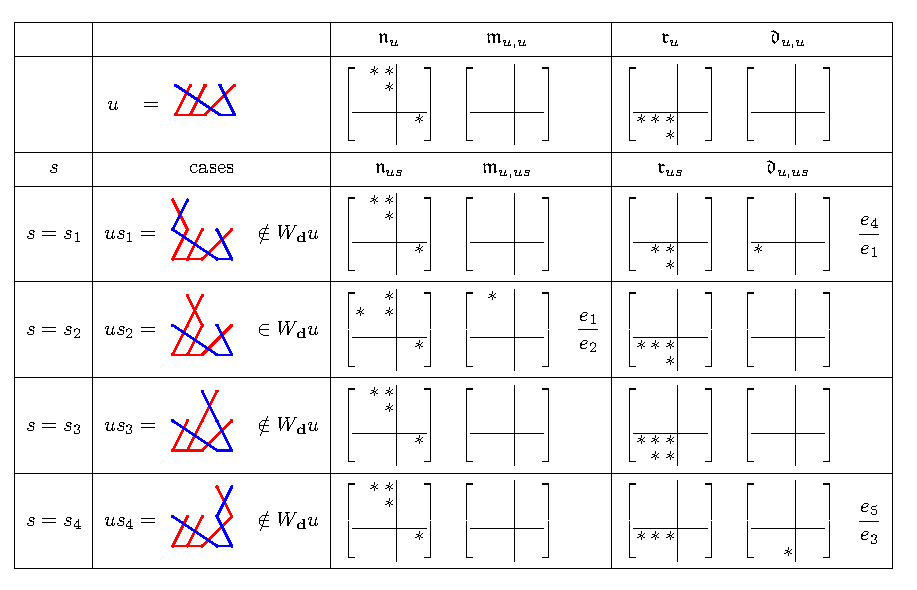
\includegraphics[width=15cm]{figures/table/table_Lie_alg.pdf}
      \caption{examples of Lie algebras}
      \label{table:Lie_alg}        
\end{table}
\end{eg}


\begin{remark}
We also have twisted notations for Lie algebras. For example,
\begin{equation*}
\begin{aligned}
  \underline{\mathfrak{n}}_{\ww,\ww'}=\;& \mathfrak{n}_{\ww,\ww\ww'},
   &&\underline{\mathfrak{m}}_{\ww,\ww'}=\; \mathfrak{m}_{\ww,\ww\ww'},
   &&
   \underline{\mathfrak{p}}_{\ww,s}=\; \mathfrak{p}_{\ww,\ww s}, \\ 
  \underline{\mathfrak{r}}_{\ww,\ww'}=\;& \mathfrak{r}_{\ww,\ww\ww'},
  &&\underline{\mathfrak{d}}_{\ww,\ww'}=\; \mathfrak{d}_{\ww,\ww\ww'}.&&  \\ 
\end{aligned}
\end{equation*}
Another twist happens when we add minus sign as the superscript:
\begin{equation*}
\begin{aligned}
  \boldsymbol{\mathfrak{b}}_{\ww}^{-} =&\boldsymbol{\mathfrak{b}}_{\ww_{\max}\ww},&& \\
  \mathfrak{b}_{\ww}^{-}=&\mathfrak{b}_{w_{\max}\ww}, & 
\mathfrak{n}_{\ww}^{-}=&\mathfrak{b}_{w_{\max}\ww}, \\
  \mathfrak{n}_{\ww,\ww''}^{-}=&\mathfrak{n}_{w_{\max}\ww,w_{\max}\ww''}, & 
\mathfrak{m}_{\ww,\ww''}^{-}=&\mathfrak{m}_{w_{\max}\ww,w_{\max}\ww''}.  \\
\end{aligned}
\end{equation*}
\end{remark}
\section{Typical variety}\label{sec:typical_variety}

In this section, we define nearly all the varieties we care about in the same spirit as Section \ref{sec:inital_case}. Their stratifications and related "Schubert" varieties will be defined in Section \ref{sec:stratification}.

Recall Setting \ref{sec:inital_case} and Definition \ref{def:flag_with_quiver}.
\subsection{Flag variety}
\begin{defn}[Absolute complete flag variety]
The absolute complete flag variety $\mathcal{F}_{\abdimvec{d}}$ is defined as 
\begin{equation*}
\begin{aligned}
  \mathcal{F}_{\abdimvec{d}}=\;& \absgp{G}_{\abdimvec{d}}/\absgp{B}_{\abdimvec{d}} \\ 
    \cong\;&  \left\{ \text{complete flags of } \mathbb{C}^{\abdimvec{d}} \right\} \\ 
      =\;& \left\{ 0 \subseteq M_1 \subseteq M_2 \subseteq \cdots \subseteq M_{\abdimvec{d}} = \mathbb{C}^{\abdimvec{d}} \;\middle|\; \dim M_j =j \right\} \\ 
       \cong\;&  \left\{ \text{Borel subgroups of } \absgp{G}_{\abdimvec{d}} \right\} \\
          =\;& \left\{ g\absgp{B}_{\abdimvec{d}}g^{-1} \;\middle|\; g \in \absgp{G}_{\abdimvec{d}} \right\} \\ 
\end{aligned}
\end{equation*}
Here, $M_i$ can have no $Q$-vector space structure.
\end{defn}

\begin{defn}[complete flag variety with flag-type dimension vector]
For a flag-type dimension vector $\ftdimvec{d}$, the flag variety $\mathcal{F}_{\ftdimvec{d}}$ is defined as
\begin{equation*}
\begin{aligned}
  \mathcal{F}_{\ftdimvec{d}}=\;&  \left\{ \text{complete flags of } V=\bigoplus_{i \in Q_0} V_i \text{ with dimension vector } \ftdimvec{d}\right\} \\ 
      =\;& \left\{ F: 0 \subseteq M_1 \subseteq M_2 \subseteq \cdots \subseteq M_{\abdimvec{d}} = V \;\middle|\; \dimv F =\ftdimvec{d} \phantom{\Big)\!\!\!} \right\}
\end{aligned}
\end{equation*}
\end{defn}

\begin{defn}[Relative complete flag variety]
The relative complete flag variety $\mathcal{F}_{\dimvec{d}}$ is defined as 
\begin{equation*}
\begin{aligned}
  \mathcal{F}_{\dimvec{d}}=\;&  \left\{ \text{complete flags of } V=\bigoplus_{i \in Q_0} V_i \right\} \\ 
      =\;& \left\{ 0 \subseteq M_1 \subseteq M_2 \subseteq \cdots \subseteq M_{\abdimvec{d}} = V \;\middle|\; \left|\dimv M_j \right| =j \phantom{\Big)\!\!\!} \right\}\\
      =\;& \bigsqcup_{\ftdimvec{d}}\mathcal{F}_{\ftdimvec{d}}
\end{aligned}
\end{equation*}
Here, $M_i$ are $Q$-vector spaces.
\end{defn}

\begin{remark}\label{rmk:action_on_flag}\
\begin{enumerate}
\item $\mathcal{F}_{\abdimvec{d}}$, $\mathcal{F}_{\ftdimvec{d}}$ and $\mathcal{F}_{\dimvec{d}}$ are smooth varieties, since
$$\mathcal{F}_{\abdimvec{d}} \cong \GL_{\abdimvec{d}}/B \qquad \mathcal{F}_{\ftdimvec{d}} \cong \prod_{i \in Q_0} \GL_{\dimvec{d}_i}/B$$
are products of usual flag varieties.
\item $\mathcal{F}_{\abdimvec{d}}$ is an $\GL_{\abdimvec{d}}$-variety, while $\mathcal{F}_{\ftdimvec{d}}$, $\mathcal{F}_{\dimvec{d}}$ are $G_{\dimvec{d}}$-varieties. The actions are induced by the actions on the vector space $V$.
\end{enumerate}
\end{remark}

We need to simplify our notations of flags.
\begin{defn}[Special flags]\label{def:special_flags}
For a basis $\{x_1, \ldots ,x_{\abdimvec{d}} \}$, denote the flag
$$F_{\{x_1, \ldots ,x_{\abdimvec{d}} \}} : 0 \subseteq \left<x_1 \right> \subseteq \left<x_1,x_2 \right>\subseteq \cdots \subseteq  \left<x_1,\ldots x_{\abdimvec{d}} \right>=V.$$
\end{defn}
For $g\in \absgp{G}_{\abdimvec{d}}$, $\ww \in \WWd$, define
\begin{equation*}
\begin{aligned}
  F_{\Id}=\;& F_{\{v_1, \ldots ,v_{\abdimvec{d}} \}} \qquad&& \in \mathcal{F}_{\dimvec{d}} \\ 
  F_{g}=\;& gF_{\Id}=F_{\{gv_1, \ldots ,gv_{\abdimvec{d}} \}} \qquad&& \in \mathcal{F}_{\abdimvec{d}} \\ 
  F_{\ww}=\;& \ww F_{\Id}=F_{\{v_{\ww(1)}, \ldots ,v_{\ww(\abdimvec{d})} \}} \qquad&& \in \mathcal{F}_{\dimvec{d}} \\ 
\end{aligned}
\end{equation*}
$F_{\Id}$ is called the \textbf{standard flag} of $V$.

Now we can define flag varieties attached to $\ww \in \WWd$.
\begin{defn}
For $\ww=wu \in \WWd$, define $\mathcal{F}_{\ww}$ as the $G_{\dimvec{d}}$-orbit of $F_{\ww}$. By the orbit-stabilizer theorem,
$$\mathcal{F}_{\ww} \cong G_{\dimvec{d}}/B_{\ww}.$$
We can generalize it a little bit: for $g \in G_{\dimvec{d}}$, $F_{g\ww} \in \mathcal{F}_{\dimvec{d}}$,
$$\mathcal{F}_{g\ww}:=G_{\dimvec{d}} \cdot F_{g\ww} \cong G_{\dimvec{d}}/B_{g\ww}=G_{\dimvec{d}}/gB_{\ww}g^{-1}.$$
\end{defn}
\begin{remark}
$F_{\ww}$ is the preferred base point of $\mathcal{F}_{\ww}$. Ignoring the base point,
$$\mathcal{F}_{\ww}=\mathcal{F}_{u}=\mathcal{F}_{\ftdimvec{d}} \quad \text{ for } \ww=wu \quad \ftdimvec{d}=\Wd \ww.$$
In fact, we are not defining new varieties; we give old varieties new names, so that we can manipulate them more freely.
\end{remark}

Like Section \ref{sec:inital_case}, we also consider the product of two flag varieties. For $g,g',g'' \in \absgp{G}_{\abdimvec{d}}$, $\ww,\ww',\ww'' \in \WWd$, denote
\begin{equation*}
\begin{aligned}
   F_{\Id,\Id}&=(F_{\Id},F_{\Id}) && \\ 
   F_{g,g''}&=(F_{g},F_{g''})\qquad & \underline{F}_{g,g'}&=F_{g,gg'}=(F_{g},F_{gg'})\\
   F_{\ww,\ww''}&=(F_{\ww},F_{\ww''}) & \underline{F}_{\ww,\ww'}&=F_{\ww,\ww\ww'}=(F_{\ww},F_{\ww\ww'})\\  
\end{aligned}
\end{equation*}

Table \ref{table:base_varieties} concludes all varieties we get until now.
\begin{table}[ht]
\centering
\[
\begin{array}{l|c|l|c}
\hline
                                                                                   &\text{base point} &                                                                                                                                                                & \text{base point}   \\ \hline
\mathcal{F}_{\abdimvec{d}} \cong \absgp{G}_{\abdimvec{d}}/\absgp{B}_{\abdimvec{d}} & F_{\Id}    & \mathcal{F}_{\abdimvec{d}} \times \mathcal{F}_{\abdimvec{d}}                                                                                                   & F_{\Id,\Id}  \\ \hline
\mathcal{F}_{\ftdimvec{d}} \cong G_{\dimvec{d}}/B_{\dimvec{d}}                     & F_u        & \mathcal{F}_{\ftdimvec{d}} \times \mathcal{F}_{\ftdimvec{d}'}                                                                                                  & F_{u,u'}     \\ \hline
\mathcal{F}_{\ww} \cong G_{\dimvec{d}}/B_{\ww}                                     & F_{\ww}    & \mathcal{F}_{\ww} \times \mathcal{F}_{\ww'}                                                                                                                    & F_{\ww,\ww'} \\ \hline
\displaystyle\mathcal{F}_{\dimvec{d}}= \bigsqcup_{\ftdimvec{d}}\mathcal{F}_{\ftdimvec{d}}       & -          & \displaystyle\mathcal{F}_{\dimvec{d}} \times \mathcal{F}_{\dimvec{d}} = \bigsqcup_{\ftdimvec{d},\ftdimvec{d}'}\mathcal{F}_{\ftdimvec{d}} \times \mathcal{F}_{\ftdimvec{d}'} & -            \\ \hline
\end{array}
\]
\caption{Base varieties and their preferred base point}
\label{table:base_varieties}
\end{table}

\subsection{Incidence variety}

Now it is time to conclude information about arrows, and construct spaces over varieties in Table \ref{table:base_varieties}.

\begin{defn}[Incidence variety]\label{def:incidence_variety}
For a quiver $Q$ with flag-type dimension vector $\ftdimvec{d}$, define
\begin{equation*}
\begin{aligned}
  \RRep_{\ftdimvec{d}}(Q):=\;& \left\{ (\rho,F) \in \Rep_{\dimvec{d}}(Q) \times \mathcal{F}_{\ftdimvec{d}}  \,\middle|\, \rho(M_j) \subseteq M_j \text{ for any } j \right\} \\
  \RRep_{\dimvec{d}}(Q):=\;& \left\{ (\rho,F) \in \Rep_{\dimvec{d}}(Q) \times \mathcal{F}_{\dimvec{d}}  \,\middle|\, \rho(M_j) \subseteq M_j \text{ for any } j \right\} \\
  =\;& \bigsqcup_{\ftdimvec{d}} \RRep_{\ftdimvec{d}}(Q)
\end{aligned}
\end{equation*}
and $\mu_{\ftdimvec{d}}$, $\pi_{\ftdimvec{d}}$, $\mu_{\dimvec{d}}$, $\pi_{\dimvec{d}}$ to be the natural morphisms from the incidence varieties to $\Rep_{\dimvec{d}}(Q)$ or flag varieties, as follows:

\begin{center}
	\begin{figure}[ht]
		\vspace{0cm}
			\parbox[t]{.5\textwidth}{\centering
			\vspace{0cm}
			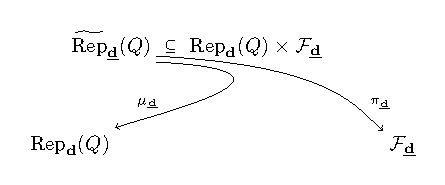
\includegraphics[width=7cm]{figures/comm_diagram/incidence_variety_1.pdf}
			}
			\parbox[t]{.5\textwidth}{\centering
			\vspace{0cm}
			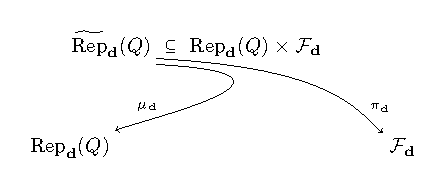
\includegraphics[width=7cm]{figures/comm_diagram/incidence_variety_2.pdf}
			}
	\end{figure}
\end{center}

\begin{remark}
For $M \in \Rep_{\dimvec{d}}(Q)$, the \textbf{Springer fiber}
$$\Flag{\ftdimvec{d}}(M):= \mu_{\ftdimvec{d}}^{-1}(M) \cong \pi_{\ftdimvec{d}}\big(\mu_{\ftdimvec{d}}^{-1}(M)\big) \subseteq \mathcal{F}_{\ftdimvec{d}}$$
records the complete flags of subrepresentations of $M$. The partial flag variety version of $\Flag{\ftdimvec{d}}(M)$ will become the key object in the second part.
\end{remark}
\end{defn}
\begin{defn}[Steinberg variety]
For quiver $Q$ with flag-type dimension vectors $\ftdimvec{d}$, $\ftdimvec{d}'$, define 
\begin{equation*}
\begin{aligned}
  \St_{\ftdimvec{d},\ftdimvec{d}'}:=\;& \RRep_{\ftdimvec{d}}(Q) \times_{\Rep_{\dimvec{d}}(Q)} \RRep_{\ftdimvec{d}'}(Q) \\
  \St_{\dimvec{d}}:=\;& \RRep_{\dimvec{d}}(Q) \times_{\Rep_{\dimvec{d}}(Q)} \RRep_{\dimvec{d}}(Q) \\
  =\;& \bigsqcup_{\ftdimvec{d},\ftdimvec{d}'} \St_{\ftdimvec{d},\ftdimvec{d}'}
\end{aligned}
\end{equation*}
$\St_{\dimvec{d}}$ is called the \textbf{Steinberg variety}.
\end{defn}
$\St_{\ftdimvec{d},\ftdimvec{d}'}$ can actually be realized as the incidence variety between $\Rep_{\dimvec{d}}(Q)$ and $\mathcal{F}_{\ftdimvec{d}} \times \mathcal{F}_{\ftdimvec{d}'}$, since
\begin{equation*}
\begin{aligned}
\St_{\ftdimvec{d},\ftdimvec{d}'}=\;& \RRep_{\ftdimvec{d}}(Q) \times_{\Rep_{\dimvec{d}}(Q)} \RRep_{\ftdimvec{d}'}(Q) \\
\subseteq \;& \left( \Rep_{\dimvec{d}}(Q) \times \mathcal{F}_{\ftdimvec{d}}  \right) 
\times_{\Rep_{\dimvec{d}}(Q)}
\left( \Rep_{\dimvec{d}}(Q) \times \mathcal{F}_{\ftdimvec{d}'}  \right) \\
\cong\;& \Rep_{\dimvec{d}}(Q) \times \mathcal{F}_{\ftdimvec{d}} \times \mathcal{F}_{\ftdimvec{d}'}
\end{aligned}
\end{equation*} 
For that reason, we denote $\mu_{\ftdimvec{d},\ftdimvec{d}'}$, $\pi_{\ftdimvec{d},\ftdimvec{d}'}$, $\mu_{\dimvec{d},\dimvec{d}}$, $\pi_{\dimvec{d},\dimvec{d}}$ as natural morphisms from $\St_{\ftdimvec{d},\ftdimvec{d}'}$, $\St_{\dimvec{d}}$ to $\Rep_{\dimvec{d}}(Q)$ or product of flag varieties, as follows:

\begin{center}
	\begin{figure}[ht]
		\vspace{0cm}
			\parbox[t]{.5\textwidth}{\centering
			\vspace{0cm}
			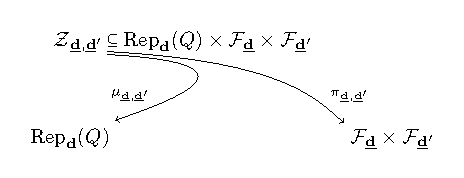
\includegraphics[width=7cm]{figures/comm_diagram/incidence_variety_3.pdf}
			}
			\parbox[t]{.5\textwidth}{\centering
			\vspace{0cm}
			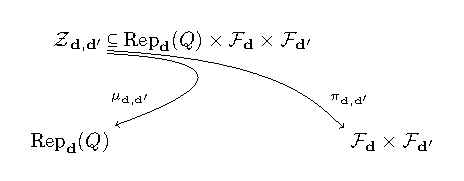
\includegraphics[width=7cm]{figures/comm_diagram/incidence_variety_4.pdf}
			}
	\end{figure}
\end{center}


\begin{remark}[Group actions]\
\begin{enumerate}
\item $\Rep_{\dimvec{d}}(Q)\subseteq \oplus_{a \in Q_1} \boldsymbol{\mathfrak{g}}_{\abdimvec{d}}$ has a natural $G_{\dimvec{d}}$-action, which is induced by the conjugation action of $G_{\dimvec{d}}$ on $\boldsymbol{\mathfrak{g}}_{\abdimvec{d}}$. We have already mentioned the $G_{\dimvec{d}}$-action on $\mathcal{F}_{\ftdimvec{d}}$ and $\mathcal{F}_{\dimvec{d}}$ in Remark \ref{rmk:action_on_flag}. Therefore, by restriction we automatically get $G_{\dimvec{d}}$-actions on $\RRep_{\ftdimvec{d}}(Q)$, $\RRep_{\dimvec{d}}(Q)$, $\St_{\ftdimvec{d},\ftdimvec{d}'}$ and $\St_{\dimvec{d}}$. All the maps we mentioned in Definition \ref{def:incidence_variety} are $G_{\dimvec{d}}$-equivariant.
\item In Section \ref{sec:Cstar_action} we will also view all the varieties as $G_{\dimvec{d}} \times \mathbb{C}^{\times}$-varieties, so we also shortly introduce $\mathbb{C}^{\times}$-action here. View $\Rep_{\dimvec{d}}(Q)$ as a $\mathbb{C}$-vector space, $\mathbb{C}^{\times}$ acts on $\Rep_{\dimvec{d}}(Q)$ by scalar multiplication. For $\mathcal{F}_{\ftdimvec{d}}$ and $\mathcal{F}_{\dimvec{d}}$, $\mathbb{C}^{\times}$ acts trivially, and by restriction we get $\mathbb{C}^{\times}$-actions on $\RRep_{\ftdimvec{d}}(Q)$, $\RRep_{\dimvec{d}}(Q)$, $\St_{\ftdimvec{d},\ftdimvec{d}'}$ and $\St_{\dimvec{d}}$. Also, all the maps we mentioned above are $\mathbb{C}^{\times}$-equivariant.
\item It may worth mentioning that $\mathcal{F}_{\dimvec{d}}$ has an $\WWd$-action which can be extended neither to $\absgp{G}_{\abdimvec{d}}$-action on $\mathcal{F}_{\dimvec{d}}$ nor to $\WWd$-action on $\RRep_{\ftdimvec{d}}(Q)$.

\end{enumerate}
\end{remark}


\section{Stratification and $T$-fixed points}\label{sec:stratification}

Natural defined varieties resemble burr puzzles, they have delicate structures and can be decomposed as relatively easy pieces. In this subsection, we will find stratifications of varieties introduced in Section \ref{sec:typical_variety}, and fix notations of orbits. We will also mention about their $T$-fixed points. These stratifications will give us a basis for the $K$-theory and cohomology theory in Chapter \ref{chap:Ktheory}, while those $T$-fixed points will give us another "basis" in Chapter \ref{chap:localization}.

\subsection{Stratification: flag variety}

We begin with $\mathcal{F}_{\abdimvec{d}}$ and $\mathcal{F}_{\abdimvec{d}} \times \mathcal{F}_{\abdimvec{d}}$, which is roughly a repetition of Section \ref{sec:inital_case}.

\begin{defn}[Twisted action]
We define the twisted $\absgp{G}_{\abdimvec{d}} \times \absgp{G}_{\abdimvec{d}}$-action on $\mathcal{F}_{\abdimvec{d}} \times \mathcal{F}_{\abdimvec{d}}$:
$$\absgp{G}_{\abdimvec{d}} \times \absgp{G}_{\abdimvec{d}} \times \mathcal{F}_{\abdimvec{d}} \times \mathcal{F}_{\abdimvec{d}} \longrightarrow \mathcal{F}_{\abdimvec{d}} \times \mathcal{F}_{\abdimvec{d}} \qquad \left( g_1,g_2,\underline{F}_{g,g'} \right) \longmapsto \underline{F}_{g_1g,g_2g'}$$
which is the same as original $\absgp{G}_{\abdimvec{d}}$-action when we restrict to $\absgp{G}_{\abdimvec{d}} \times \{\Id \}$-action. Other $G \times G$-actions on $\mathcal{F} \times \mathcal{F}$ are defined in a similar way.
\end{defn}

\begin{defn}[Stratifications of $\mathcal{F}_{\abdimvec{d}}$ and $\mathcal{F}_{\abdimvec{d}} \times \mathcal{F}_{\abdimvec{d}}$]
For $\ww,\ww' \in \WWd$, we define
\begin{equation*}
\begin{aligned}
  \Vcell_{\ww}=\;& \absgp{B}_{\abdimvec{d}} \cdot F_{\ww} \qquad&& \subseteq \mathcal{F}_{\abdimvec{d}} \\ 
  \VVcell_{\ww,\ww'}=\;& \left(\absgp{B}_{\abdimvec{d}} \times \absgp{B}_{\abdimvec{d}}\right) \cdot \underline{F}_{\ww,\ww'} && \subseteq \mathcal{F}_{\abdimvec{d}} \times \mathcal{F}_{\abdimvec{d}} \\ 
  \VVcell_{\ww'}=\;& \absgp{G}_{\abdimvec{d}} \cdot \underline{F}_{\Id,\ww'} && \subseteq \mathcal{F}_{\abdimvec{d}} \times \mathcal{F}_{\abdimvec{d}} \\ 
\end{aligned}
\end{equation*}
as $\absgp{B}_{\abdimvec{d}}$-orbit, $\absgp{B}_{\abdimvec{d}} \times \absgp{B}_{\abdimvec{d}}$-orbit, $\absgp{G}_{\abdimvec{d}}$-orbit of $\mathcal{F}_{\abdimvec{d}}$, $\mathcal{F}_{\abdimvec{d}} \times \mathcal{F}_{\abdimvec{d}}$, $\mathcal{F}_{\abdimvec{d}} \times \mathcal{F}_{\abdimvec{d}}$, respectively.
\end{defn}

By Bruhat-decomposition, we are able to show
$$\mathcal{F}_{\abdimvec{d}}= \bigsqcup_{\ww} \Vcell_{\ww} \qquad \mathcal{F}_{\abdimvec{d}} \times \mathcal{F}_{\abdimvec{d}} = \bigsqcup_{\ww'} \VVcell_{\ww'} = \bigsqcup_{\ww,\ww'} \VVcell_{\ww,\ww'}.$$
We also realize these orbits as quotients of algebraic groups by the orbit-stabilizer theorem, as follows:
\begin{equation*}
\begin{aligned}
  \Vcell_{\ww}\cong\;& \absgp{B}_{\abdimvec{d}} /\left(  \absgp{B}_{\abdimvec{d}} \cap \absgp{B}_{\ww} \right) \qquad&&  \cong \mathbb{A}^{l(\ww)} \\ 
  \VVcell_{\ww,\ww'}\cong\;& \left(\absgp{B}_{\abdimvec{d}} \times \absgp{B}_{\abdimvec{d}}\right) / \left(\absgp{B}_{\abdimvec{d}} \cap \absgp{B}_{\ww} \times \absgp{B}_{\abdimvec{d}} \cap \absgp{B}_{\ww'}\right)&& \cong \mathbb{A}^{l(\ww)+l(\ww')}  \\ 
  \VVcell_{\ww'}\cong\;& \absgp{G}_{\abdimvec{d}} /\left(  \absgp{B}_{\abdimvec{d}} \cap \absgp{B}_{\ww'} \right) && \cong \mathbb{A}^{l(\ww')}\text{-bundle over }\mathcal{F}_{\abdimvec{d}}  \\ 
\end{aligned}
\end{equation*}

Similar stratifications happen for $\mathcal{F}_{u}$ and $\mathcal{F}_{\dimvec{d}}$.

\begin{defn}[Stratifications of $\mathcal{F}_{u}$ and $\mathcal{F}_{u} \times \mathcal{F}_{u'}$]
For $u,u' \in \MinWd$, $w,w' \in \Wd$, we define
\begin{equation*}
\begin{aligned}
  \Omcell_{w}^{u}=\;& B_{\dimvec{d}} \cdot F_{wu} \qquad&& \subseteq \mathcal{F}_{u} \\ 
  \OOmcell_{w,w'}^{u,u'}=\;& \left(B_{\dimvec{d}} \times B_{\dimvec{d}}\right) \cdot \left( F_{wu}, F_{ww'u'} \right)  && \subseteq \mathcal{F}_{u} \times \mathcal{F}_{u'}\\ 
  \OOmcell_{w'}^{u,u'}=\;&  G_{\dimvec{d}} \cdot \left( F_{u}, F_{w'u'} \right) && \subseteq \mathcal{F}_{u} \times \mathcal{F}_{u'} \\ 
\end{aligned}
\end{equation*}
as $B_{\dimvec{d}}$-orbit, $B_{\dimvec{d}} \times B_{\dimvec{d}}$-orbit, $G_{\dimvec{d}}$-orbit of $\mathcal{F}_{u}$, $\mathcal{F}_{u} \times \mathcal{F}_{u'}$, $\mathcal{F}_{u} \times \mathcal{F}_{u'}$, respectively.
\end{defn}

By Bruhat decomposition, we are again able to show
$$\mathcal{F}_{u}= \bigsqcup_{w} \Omcell_{w}^{u} \qquad \mathcal{F}_{u} \times \mathcal{F}_{u'} = \bigsqcup_{w'} \OOmcell_{w'}^{u,u'} = \bigsqcup_{w,w'} \OOmcell_{w,w'}^{u,u'}$$
and
\begin{equation*}
\begin{aligned}
  \Omcell_{w}^{u}\cong\;& B_{\dimvec{d}} /\left(  B_{\dimvec{d}} \cap B_{w} \right) \qquad&&  \cong \mathbb{A}^{l(w)} \\ 
  \OOmcell_{w,w'}^{u,u'}\cong\;& \left(B_{\dimvec{d}} \times B_{\dimvec{d}}\right) / \left(B_{\dimvec{d}} \cap B_{w} \times B_{\dimvec{d}} \cap B_{w'}\right)&& \cong \mathbb{A}^{l(w)+l(w')}  \\ 
  \OOmcell_{w'}^{u,u'}\cong\;& G_{\dimvec{d}} /\left(  B_{\dimvec{d}} \cap B_{w'} \right) && \cong \mathbb{A}^{l(w')}\text{-bundle over }\mathcal{F}_{u}  \\ 
\end{aligned}
\end{equation*}

\begin{defn}[Stratifications of $\mathcal{F}_{\dimvec{d}}$ and $\mathcal{F}_{\dimvec{d}} \times \mathcal{F}_{\dimvec{d}}$]
For $\ww,\ww' \in \WWd$, we define
\begin{equation*}
\begin{aligned}
  \Ocell_{\ww}=\;& B_{\dimvec{d}} \cdot F_{\ww} \qquad&&\subseteq \mathcal{F}_{\ww}&& \subseteq \mathcal{F}_{\dimvec{d}} \\ 
  \OOcell_{\ww,\ww'}=\;& \left(B_{\dimvec{d}} \times B_{\dimvec{d}}\right) \cdot \underline{F}_{\ww,\ww'} && \subseteq \mathcal{F}_{\ww} \times \mathcal{F}_{\ww\ww'} && \subseteq \mathcal{F}_{\dimvec{d}} \times \mathcal{F}_{\dimvec{d}}\\ 
  \OOcell_{\ww'}=\;& \bigsqcup_{u} G_{\dimvec{d}} \cdot \underline{F}_{u,\ww'} && \subseteq \bigsqcup_{u}\mathcal{F}_{u} \times \mathcal{F}_{u\ww'}\hspace{-1cm}&& \subseteq \mathcal{F}_{\dimvec{d}} \times \mathcal{F}_{\dimvec{d}} \\ 
\end{aligned}
\end{equation*}
as $B_{\dimvec{d}}$-orbit, $B_{\dimvec{d}} \times B_{\dimvec{d}}$-orbit, (union of) $G_{\dimvec{d}}$-orbit of $\mathcal{F}_{\dimvec{d}}$, $\mathcal{F}_{\dimvec{d}} \times \mathcal{F}_{\dimvec{d}}$, $\mathcal{F}_{\dimvec{d}} \times \mathcal{F}_{\dimvec{d}}$, respectively.
\end{defn}
Notice that $\Ocell_{\ww}$, $\OOcell_{\ww,\ww'}$, $\OOcell_{\ww'}$ are preimages of $\Vcell_{\ww}$, $\VVcell_{\ww,\ww'}$, $\VVcell_{\ww'}$ under the maps
$$\mathcal{F}_{\dimvec{d}} \hookrightarrow  \mathcal{F}_{\abdimvec{d}} \qquad \mathcal{F}_{\dimvec{d}} \times \mathcal{F}_{\dimvec{d}} \hookrightarrow  \mathcal{F}_{\abdimvec{d}} \times \mathcal{F}_{\abdimvec{d}}.$$
Therefore, 
$$\mathcal{F}_{\dimvec{d}}= \bigsqcup_{\ww} \Ocell_{\ww} \qquad \mathcal{F}_{\dimvec{d}} \times \mathcal{F}_{\dimvec{d}} = \bigsqcup_{\ww'} \OOcell_{\ww'} = \bigsqcup_{\ww,\ww'} \OOcell_{\ww,\ww'}.$$

%Some stratifications are quite compatible with the connected component of $\mathcal{F}_{\dimvec{d}}$, so we give new names for them.



We still need to care about symbols. For $\ww=wu$, $\ww'=w'u'$, denote $uw'u'=\tilde{w}\tilde{u}$ for $\tilde{w}' \in \Wd$, $\tilde{u} \in \MinWd$, then
$$\underline{F}_{\ww,\ww'}= \left( F_{\ww}, F_{\ww\ww'}  \right)= \left( F_{wu}, F_{wuw'u'}  \right)= \left( F_{wu}, F_{w\tilde{w}\tilde{u}}  \right) \in \mathcal{F}_{u} \times \mathcal{F}_{\tilde{u}}.$$
This incompatibility comes from our twisted $G_{\dimvec{d}} \times G_{\dimvec{d}}$-actions. In particular, denote
$$\OOcell_{\ww'}^{u}:= G_{\dimvec{d}} \cdot \underline{F}_{u,\ww'}\subseteq \mathcal{F}_{u} \times \mathcal{F}_{\tilde{u}},$$
we have $\OOcell_{\ww'}=\sqcup_{u} \OOcell_{\ww'}^{u}$ and identifications
\begin{equation}\label{eq:identification}
\Ocell_{\ww}=\Omcell_{w}^{u} \qquad \OOcell_{\ww,\ww'}=\OOmcell_{w,\tilde{w}}^{u,\tilde{u}} \qquad \OOcell_{\ww'}^{u}=\OOmcell_{\tilde{w}}^{u,\tilde{u}}.\tag{$\star$}
\end{equation}

We can also describe the closure of orbits, for example,
\begin{equation*}
  \overline{\Omcell}_{w}^{u}= \bigsqcup_{x\leq w}\Omcell_{x}^{u}  \qquad
  \overline{\OOmcell}_{w,w'}^{u,u'}=\bigsqcup_{x \leq w, x'\leq w'} \OOmcell_{x,x'}^{u,u'} \qquad
  \overline{\OOmcell}_{w'}^{u,u'}=\bigsqcup_{x'\leq w'} \OOmcell_{x'}^{u,u'} \\ 
\end{equation*}
Especially, for any $s \in \Pi_{\dimvec{d}}$, $u,u' \in \MinWd$, we have
$$\overline{\OOmcell}_{s}^{u,u'} = \OOmcell_{s}^{u,u'} \sqcup \OOmcell_{\Id}^{u,u'} \cong G_{\dimvec{d}} \times^{B_{\dimvec{d}}} \left( P_{\Id,s} / B_{\dimvec{d}} \right)$$
when we work over base point $F_{u,u'}$. If we work over different base points, we will get different isomorphisms, as follows:
\begin{equation*}
\begin{aligned}
 \overline{\OOmcell}_{s}^{u,u'} = \OOmcell_{\Id}^{u,u'}\sqcup \OOmcell_{s}^{u,u'} \cong\;& 
  G_{\dimvec{d}} /(B_w \cap B_{ws} ) &&\sqcup G_{\dimvec{d}}/B_w \\ 
  \cong\;&  G_{\dimvec{d}} \times^{B_w} \big(B_w/(B_w \cap B_{ws})\big)\hspace{-0.4cm} &&\sqcup G_{\dimvec{d}} \times^{B_w} (B_w/B_w) \\ 
  \cong\;& G_{\dimvec{d}} \times^{B_w} (B_w sB_w/B_w) &&\sqcup G_{\dimvec{d}} \times^{B_w} (B_w/B_w)  \\ 
  \cong\;& G_{\dimvec{d}} \times^{B_w} (\underline{P}_{w,s}/B_w)&& \qquad \text{ base point }F_{wu,wu'}\\ 
  \cong\;& G_{\dimvec{d}} \times^{B_w} (\underline{P}_{w,s}/B_{ws})&& \qquad \text{ base point }F_{wu,wsu'}\\ 
\end{aligned}
\end{equation*}

Closures of $\OOcell$-cells are obtained by identifications \eqref{eq:identification}. To illustrate it, we compute $\overline{\OOcell}_s$ by hand. Let $\ww'=s, us=\tilde{w}\tilde{u}$,
 
\begin{equation*}
\begin{aligned}
 \overline{\OOcell}_{s} = \;&\bigsqcup_u \overline{\OOcell}_{s}^{u} = \bigsqcup_u \overline{\OOmcell}_{\tilde{w}}^{u,\tilde{u}}\\
 =\;& \left(\bigsqcup_{u:usu^{-1} \in \Wd} \overline{\OOmcell}_{usu^{-1}}^{u,u}\right) \sqcup \left(\bigsqcup_{u:usu^{-1} \notin \Wd} \overline{\OOmcell}_{\Id}^{u,us}\right)\\
 =\;& \left(\bigsqcup_{u:usu^{-1} \in \Wd} \OOmcell_{usu^{-1}}^{u,u}\right) \sqcup \left(\bigsqcup_{u:usu^{-1} \notin \Wd} \OOmcell_{\Id}^{u,us}\right) \sqcup \left(\bigsqcup_{u:usu^{-1} \in \Wd} \OOmcell_{\Id}^{u,u}\right)\\
 =\;&\OOcell_{s} \sqcup \left(\bigsqcup_{u:usu^{-1} \in \Wd} \OOcell_{\Id}^{u}\right)
\end{aligned}
\end{equation*}

We restrict the result of $\overline{\OOmcell}_{s}^{u,u'}$ to $\overline{\OOcell}_{s}^{u}$ in Lemma \ref{lem:iso_of_orbits}.

\begin{lemma}\label{lem:iso_of_orbits}
For $\ww=wu \in \WWd$, $s\in \Pi$ such that $\ww s \ww^{-1} \in \Wd$, we have isomorphisms of $G_{\dimvec{d}}$-varieties
\begin{equation*}
\begin{aligned}
& G_{\dimvec{d}} \times^{B_{\ww}} (\underline{P}_{\ww,s}/B_{\ww}) \longrightarrow \overline{\OOcell}_{s}^{u} \qquad && (g,p) \longmapsto (g \cdot F_{\ww}, gp \cdot F_{\ww})\\
& G_{\dimvec{d}} \times^{B_{\ww}} (\underline{P}_{\ww,s}/B_{\ww s}) \longrightarrow \overline{\OOcell}_{s}^{u} \qquad && (g,p) \longmapsto (g \cdot F_{\ww}, gp \cdot F_{\ww s})\\
\end{aligned}
\end{equation*}
\end{lemma}
\begin{proof}
Notice that when $\ww s \ww^{-1} \in \Wd$, $\OOcell_{s}^{u}=\OOmcell_{usu^{-1}}^{u,u}$. Therefore, 
\begin{equation*}
\begin{aligned}
 \overline{\OOcell}_{s}^{u}=\overline{\OOmcell}_{usu^{-1}}^{u,u} \cong\;& 
 \begin{cases}
 G_{\dimvec{d}} \times^{B_w} (\underline{P}_{w,usu^{-1}}/B_w) & \text{ base point }F_{wu,wu} \\
 G_{\dimvec{d}} \times^{B_w} (\underline{P}_{w,usu^{-1}}/B_{wusu^{-1}}) & \text{ base point }F_{wu,wus} 
 \end{cases} \\ 
  \cong\;& 
  \begin{cases}
  G_{\dimvec{d}} \times^{B_{\ww}} (\underline{P}_{\ww,s}/B_{\ww}) & \qquad\text{ base point }F_{\ww,\ww} \\
  G_{\dimvec{d}} \times^{B_{\ww}} (\underline{P}_{\ww,s}/B_{\ww s}) & \qquad\text{ base point }F_{\ww,\ww s} 
  \end{cases} \\ 
\end{aligned}
\end{equation*}
\\[-2\baselineskip]
\end{proof}





After so many notations are introduced rapidly, an enlightening example is needed here.
\begin{eg}[Follows Example \ref{eg:3-case-1}]\label{eg:3-case-2}
Here, $\WWd=S_3$, $\Wd=S_1 \times S_2$,
$$\ww=ts=t \cdot s, \qquad \ww'=s=\Id \cdot s,\qquad \ww\ww'=t=t \cdot \Id.$$

$\mathcal{F}_{\dimvec{d}}$ has $3$ connected components, each of them has $2$ $B_{\dimvec{d}}$-orbits;

 $\mathcal{F}_{\dimvec{d}} \times \mathcal{F}_{\dimvec{d}}$ has $9$ connected components, each of them has $4$ $B_{\dimvec{d}} \times B_{\dimvec{d}}$-orbits.
\begin{table}[ht]
  \vspace{0cm}
    \centering  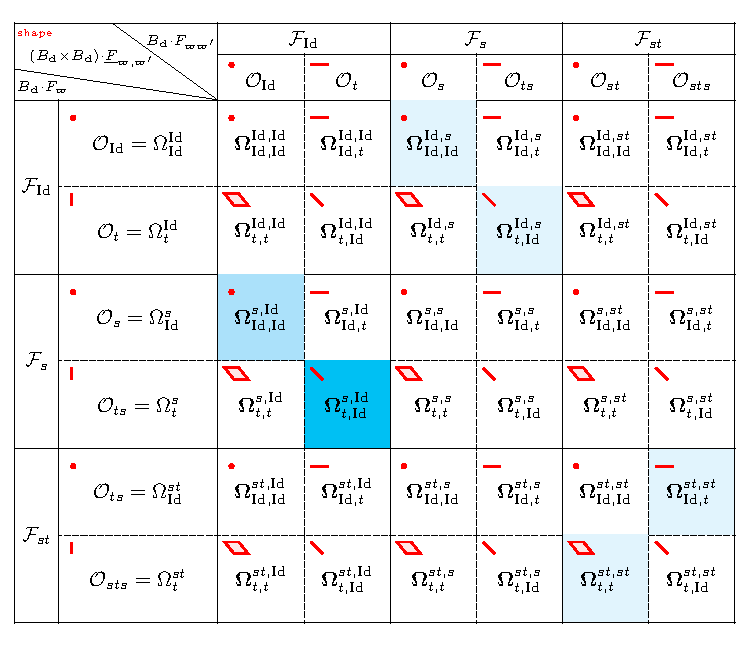
\includegraphics[width=12.8cm]{figures/table/table_2.pdf}
        \caption{stratifications of $\mathcal{F}_{\dimvec{d}}\times \mathcal{F}_{\dimvec{d}}$}
        \label{table:stratifications_of_FdFd}
\end{table}
We have given every orbit a name, and other spaces are finite union of these orbits. For example,
\begin{equation*}
\begin{aligned}
  \OOcell_{ts,s}=\;& \OOmcell_{t,\Id}^{s,\Id} \\ 
  \OOcell_{s}^{s}=\;& \OOmcell_{\Id}^{s,\Id} = \OOmcell_{\Id,\Id}^{s,\Id} \sqcup \OOmcell_{t,\Id}^{s,\Id} \\ 
  \OOcell_{s}=\;& \OOcell_{s}^{s} \sqcup \OOcell_{s}^{\Id} \sqcup \OOcell_{s}^{st} \\   
  =\;& \OOcell_{s}^{s} \sqcup \OOcell_{s}^{\Id} \sqcup \OOcell_{s}^{st} \\  
  =\;& \OOmcell_{\Id}^{s,\Id} \sqcup \OOmcell_{\Id}^{\Id,s} \sqcup \OOmcell_{\Id}^{st,st}
   \\  
  =\;& \OOmcell_{\Id,\Id}^{s,\Id} \sqcup \OOmcell_{t,\Id}^{s,\Id} \sqcup \OOmcell_{\Id,\Id}^{\Id,s} \sqcup  \OOmcell_{t,\Id}^{\Id,s} \sqcup \OOmcell_{\Id,\Id}^{st,st} \sqcup \OOmcell_{t,\Id}^{st,st}
   \\  
\end{aligned}
\end{equation*}
Their closures are also clear from the table, for example, 
$$\overline{\OOcell}_s=\OOcell_{s} \sqcup \OOmcell_{\Id}^{st,st}$$
contains $8$ $B_{\dimvec{d}} \times B_{\dimvec{d}}$-orbits.
\end{eg}


\subsection{Stratification: incidence variety}
Now comes the stratifications of incidence varieties. Those stratifications are produced by taking the preimage of stratifications on base spaces. They are relatively easy to obtain, while their closures are quite difficult to analyze.

\begin{defn}[Stratifications of incidence varieties]
For $\ww=wu$, $\ww'=w'u' \in \WWd$, denote $uwu' =\tilde{w}\tilde{u}$, $\ftdimvec{d}=\Wd u$, $\ftdimvec{d}'=\Wd u'$, $\widetilde{\ftdimvec{d}}=\Wd \tilde{u}$, we define
\begin{equation*}
\begin{aligned}
  \preimage{\Omcell}_{w}^{u}:=\;& \pi_{\ftdimvec{d}}^{-1}(\Omcell_{w}^{u})&& \subseteq \RRep_{\ftdimvec{d}}(Q) \\ 
  \preimage{\OOmcell}_{w,w'}^{u,u'}:=\;& \pi_{\ftdimvec{d},\ftdimvec{d}'}^{-1}(\OOmcell_{w,w'}^{u,u'})&& \subseteq \St_{\ftdimvec{d},\ftdimvec{d}'} \\ 
  \preimage{\OOmcell}_{w'}^{u,u'}:=\;& \pi_{\ftdimvec{d},\ftdimvec{d}'}^{-1}(\OOmcell_{w'}^{u,u'})&& \subseteq \St_{\ftdimvec{d},\ftdimvec{d}'} \\[3mm]
  \preimage{\OOcell}_{\ww'}^{u}:=\;& \pi_{\ftdimvec{d},\widetilde{\ftdimvec{d}}}^{-1}(\OOcell_{\ww'}^{u}) = \preimage{\OOmcell}_{\tilde{w}}^{u,\tilde{u}}\hspace{1cm}&& \subseteq \St_{\ftdimvec{d},\widetilde{\ftdimvec{d}}}  \\[3mm]
  \preimage{\Ocell}_{\ww}:=\;& \pi_{\dimvec{d}}^{-1}(\Ocell_{\ww})&& \subseteq \RRep_{\dimvec{d}}(Q) \\ 
  \preimage{\OOcell}_{\ww,\ww'}:=\;& \pi_{\dimvec{d},\dimvec{d}'}^{-1}(\OOcell_{\ww,\ww'})&& \subseteq \St_{\dimvec{d}} \\ 
  \preimage{\OOcell}_{\ww'}:=\;& \pi_{\dimvec{d},\dimvec{d}'}^{-1}(\OOcell_{\ww'})&& \subseteq \St_{\dimvec{d}} \\ 
\end{aligned}
\end{equation*}
\end{defn}


It is not hard to see that they are stratifications:
\begin{equation*}
\begin{aligned}
  \RRep_{\ftdimvec{d}}(Q)=\;& \bigsqcup_{\ww} \preimage{\Omcell}_{w}^{u} \qquad &  \St_{\ftdimvec{d},\ftdimvec{d}'} =\;& \bigsqcup_{w} \preimage{\OOmcell}_{w'}^{u,u'} = \bigsqcup_{w,w'} \preimage{\OOmcell}_{w,w'}^{u,u'}  \\
  \RRep_{\dimvec{d}}(Q)=\;& \bigsqcup_{\ww} \preimage{\Ocell}_{\ww} \qquad &  \St_{\dimvec{d}} =\;& \bigsqcup_{\ww'} \preimage{\OOcell}_{\ww'} = \bigsqcup_{\ww,\ww'} \preimage{\OOcell}_{\ww,\ww'}  \\
\end{aligned}
\end{equation*}

\begin{proposition}\label{prop:strataffine}
Those stratifications are affine spaces over corresponding base spaces. To be precise,
\begin{equation*}
\begin{aligned}
  \preimage{\Omcell}_{w}^{u}=\;& \mathfrak{r}_{wu}\text{-bundle over }\Omcell_{w}^{u}  \\ 
  \preimage{\OOmcell}_{w,w'}^{u,u'}=\;&\mathfrak{r}_{wu,ww'u'}\text{-bundle over }\OOmcell_{w,w'}^{u,u'} \\ 
  \preimage{\OOmcell}_{w'}^{u,u'}=\;&\mathfrak{r}_{u,w'u'}\text{-bundle over }\OOmcell_{w'}^{u,u'} \\[3mm]
  \preimage{\OOcell}_{\ww'}^{u}=\;&\underline{\mathfrak{r}}_{u,\ww'}\text{-bundle over }\OOcell_{\ww'}^{u}  \\[3mm]
  \preimage{\Ocell}_{\ww}=\;&\mathfrak{r}_{\ww}\text{-bundle over }\Ocell_{\ww} \\ 
  \preimage{\OOcell}_{\ww,\ww'}=\;&\underline{\mathfrak{r}}_{\ww,\ww'}\text{-bundle over }\OOcell_{\ww,\ww'} \\ 
  \preimage{\OOcell}_{\ww'}=\;&\underline{\mathfrak{r}}_{\Id,\ww'}\text{-bundle over }\OOcell_{\ww'} \\ 
\end{aligned}
\end{equation*}
\end{proposition}

\begin{proof}
The fibers are all computed over the preferred base point. The group action induces the isomorphism between different fibers, and lift affine local charts on base space (viewed as group quotient) to the local charts of fiber bundles. 
\end{proof}

We will frequently use closures of some stratifications, so we give them names.

\begin{defn}
We define
\begin{equation*}
\begin{aligned}
  \St_{w'}^{u,u'}:=\;& \overline{\preimage{\OOmcell}}_{w'}^{u,u'} && \subseteq \hspace{7mm}\St^{u,u'}:= \St_{\ftdimvec{d},\ftdimvec{d}'}, \\
  \St_{\ww'}:=\;& \overline{\preimage{\OOcell}}_{\ww'} && \subseteq \phantom{\hspace{7mm} \St^{u,u'}:=}\St_{\dimvec{d}}.
\end{aligned}
\end{equation*}
\end{defn}

\begin{proposition}[Properties of the closure]
$\St_{\ww'}$ is a Zarisky-locally trivial cone bundle over $\mathcal{F}_{\dimvec{d}} \times \mathcal{F}_{\dimvec{d}}$. To be precise, under the map
$$\pi_{\dimvec{d},\dimvec{d},\ww'}: \St_{\ww'} \longrightarrow \mathcal{F}_{\dimvec{d}} \times \mathcal{F}_{\dimvec{d}},$$
for any $x,x' \in \WWd$, $\pi_{\dimvec{d},\dimvec{d},\ww'}^{-1}(\OOcell_{x,x'})$ is a trivial fiber bundle over $\OOcell_{x,x'}$, whose fibers are cones.
\end{proposition}

Notice that
\begin{equation*}
\begin{aligned}
  \St_{w'}^{u,u'}:=\;& \overline{\preimage{\OOmcell}}_{w'}^{u,u'} && \subseteq \hspace{7mm}\preimage{\overline{\OOmcell}}_{w'}^{u,u'}:= \pi_{\ftdimvec{d},\ftdimvec{d}'}^{-1}\left( \overline{\OOmcell}_{w'}^{u,u'} \right), \\
  \St_{\ww'}:=\;& \overline{\preimage{\OOcell}}_{\ww'} && \subseteq \hspace{7mm} \preimage{\overline{\OOcell}}_{\ww'} :=\pi_{\dimvec{d},\dimvec{d}}^{-1}\left( \overline{\OOcell}_{\ww'} \right).
\end{aligned}
\end{equation*}
Even though these inclusions are usually not equalities, we can still say something when the length of $w'$ or $\ww'$ is small. For example,
\begin{equation*}
\begin{aligned}
&\St_{\Id}^{u,u'}=\preimage{\OOmcell}_{\Id}^{u,u'} \\ 
&\St_{\Id}=\preimage{\OOcell}_{\Id}\\
\preimage{\OOmcell}_{s}^{u,u'}\sqcup \OOmcell_{\Id}^{u,u'} \subseteq &\St_{s}^{u,u'} \subseteq \preimage{\OOmcell}_{s}^{u,u'}\sqcup \preimage{\OOmcell}_{\Id}^{u,u'} \qquad &(s \in \Pi_{\dimvec{d}})\\
 \preimage{\OOcell}_{s} \sqcup \left(\bigsqcup_{u:usu^{-1} \in \Wd}\OOcell_{\Id}^{u}\right) \subseteq& \St_{s} \subseteq \preimage{\OOcell}_{s} \sqcup \left(\bigsqcup_{u:usu^{-1} \in \Wd}\preimage{\OOcell}_{\Id}^{u}\right) \qquad &(s \in \Pi_{\phantom{d}})
\end{aligned}
\end{equation*}

\begin{proposition}\label{prop:vector_bundle_Z_s}
$\St_s$ is a Zarisky-locally trivial vector bundle over $\overline{\OOcell}_s$, with fiber $\mathfrak{r}_{u,us}$ at point $\underline{F}_{u,s}$.
\end{proposition}
\begin{proof}
This is claimed in \cite[2.20(c)]{varagnolo2011canonical}. In fact, we have a $G_{\dimvec{d}}$-equivariant morphism
$$\phi: G_{\dimvec{d}} \times^{B_u} \left(  \underline{P}_{u,s}/B_{us} \times \underline{\mathfrak{r}}_{u,s} \right) \hookrightarrow \Rep_{\dimvec{d}}(Q) \times \mathcal{F}_{\dimvec{d}} \times \mathcal{F}_{\dimvec{d}} \qquad (g,p,x) \longmapsto (gx, g \cdot F_u, gp \cdot F_{us})$$
which realized $G_{\dimvec{d}} \times^{B_u} \left(  \underline{P}_{u,s}/B_{us} \times \underline{\mathfrak{r}}_{u,s} \right)$ as a closed subset of $\Rep_{\dimvec{d}}(Q) \times \mathcal{F}_{\dimvec{d}}$. In the meantime, the open dense subset $$G_{\dimvec{d}} \times^{B_u} \left(  B_{us}sB_{us}/B_{us}\times \underline{\mathfrak{r}}_{u,s} \right) \subseteq G_{\dimvec{d}} \times^{B_u} \left(  \underline{P}_{u,s}/B_{us}\times \underline{\mathfrak{r}}_{u,s} \right)$$
 is identified with $\preimage{\OOcell}_{s}^{u}$ by $\phi$. Therefore, $\phi$ identifies $\St_{s}^{u,\tilde{u}}$ with the vector bundle $G_{\dimvec{d}} \times^{B_u} \left(  \underline{P}_{u,s}/B_{us} \times \underline{\mathfrak{r}}_{u,s} \right)$ over $\overline{\OOcell}_{s}^{u}$, with fiber $\underline{\mathfrak{r}}_{u,s}=\mathfrak{r}_{u,us}$.
\end{proof}

\begin{remark}\label{rmk:vector_bundle_O_s}
By the same method, one can show that $\overline{\preimage{\Ocell}}_{s}$ is a Zarisky-locally trivial vector bundle over $\overline{\Ocell}_s$, with fiber $\mathfrak{r}_{s}$ at point $F_{s}$.
\end{remark}
We end this subsection by Table \ref{table:orbit}:
\begin{table}[ht]
  \vspace{0cm}
    \centering  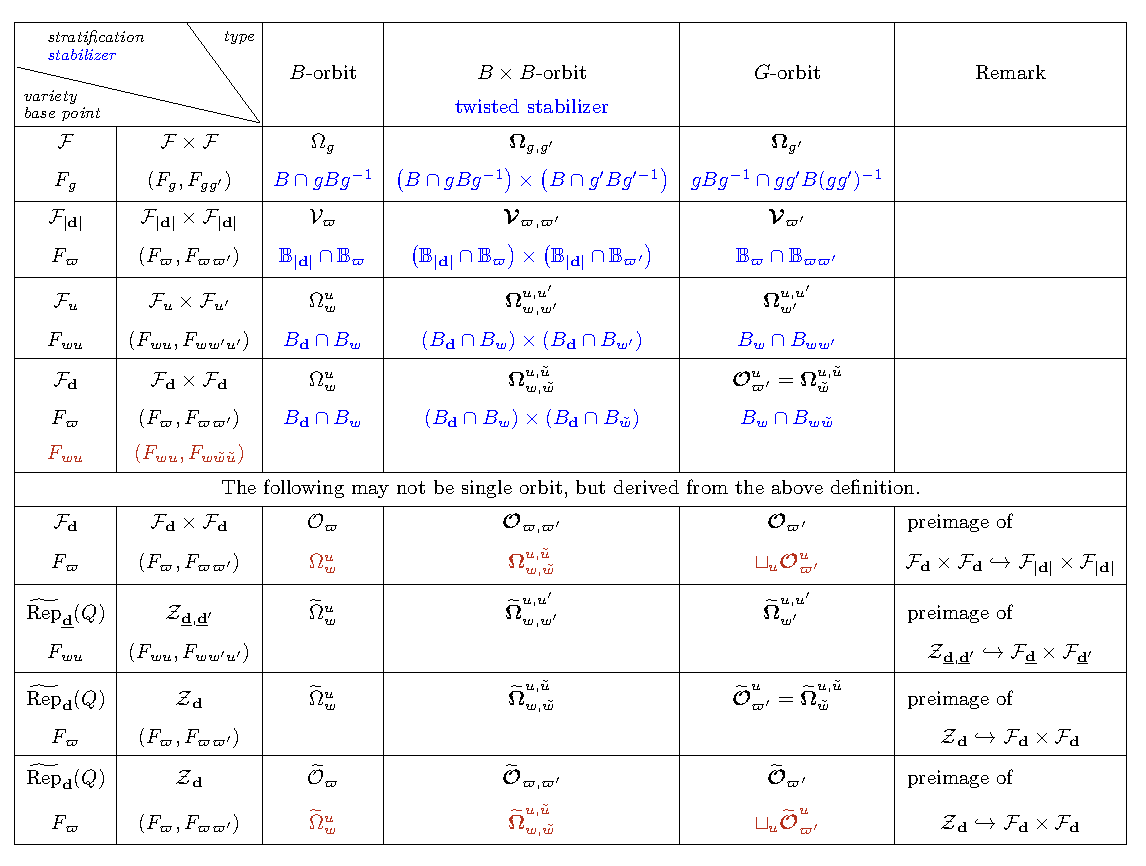
\includegraphics[width=15cm]{figures/table/table_orbit.pdf}
      \caption{stratifications of typical varieties}
      \label{table:orbit}        
\end{table}

\subsection{$T$-fixed points}

Compare with stratifications, $T$-fixed points are easy to compute and have clear structures. Somewhat surprisingly, these $T$-fixed points encode most information of varieties.

Recall that the $T$-fixed points of a complete flag variety $\mathcal{F}$ are exactly those coordinate flags $\left\{ F_w \,\middle|\, w \in W \right\}$. For absolute or relative flag varieties, we have similar results:
$$\mathcal{F}_{\abdimvec{d}}^{\absgp{T}_{\abdimvec{d}}} = \mathcal{F}_{\dimvec{d}}^{T_{\dimvec{d}}}= \left\{ F_{\ww} \,\middle|\, \ww \in \WWd \right\} \qquad \mathcal{F}_u^{T_{\dimvec{d}}} = \left\{ F_{wu} \,\middle|\, w \in \Wd \right\}$$ 
For $\Rep_{\dimvec{d}}(Q)$, we get
$$\big(\!\Rep_{\dimvec{d}}(Q) \big)^{T_{\dimvec{d}}} = \bigoplus_{a \in Q_1} \bigg( \Hom \left(\mathbb{C}^{\dimvec{d}_{s(a)}},\mathbb{C}^{\dimvec{d}_{t(a)}}\right) \bigg)^{T_{\dimvec{d}}} =\{ \rho_0 \}$$
where $\rho_0$ is the zero representation in $\Rep_{\dimvec{d}}(Q)$.

Combining these two results, one can easily describe $T$-fixed points of varieties constructed over them:
\begin{equation*}
\begin{aligned}
  \left(\mathcal{F}_{\abdimvec{d}} \times \mathcal{F}_{\abdimvec{d}}\right)^{\absgp{T}_{\abdimvec{d}}}=\;& \left\{  (F_{\ww},F_{\ww'}) \,\middle|\,  \ww,\ww' \in \WWd  \right\} \\ 
  \left(\mathcal{F}_{u} \times \mathcal{F}_{u'}\right)^{T_{\dimvec{d}}}=\;&  \left\{  (F_{wu},F_{w'u'}) \,\middle|\,  w,w' \in \Wd  \right\} \\ 
  \left(\mathcal{F}_{\dimvec{d}} \times \mathcal{F}_{\dimvec{d}}\right)^{T_{\dimvec{d}}}=\;&  \left\{  (F_{\ww},F_{\ww'}) \,\middle|\,  \ww,\ww' \in \WWd  \right\} \\ 
  \left(\RRep_{\ftdimvec{d}}(Q)\right)^{T_{\dimvec{d}}}=\;& \left\{  (\rho_0,F_{wu}) \,\middle|\,  w \in \Wd  \right\} \\ 
  \left(\RRep_{\dimvec{d}}(Q)\right)^{T_{\dimvec{d}}}=\;& \left\{  (\rho_0,F_{\ww}) \,\middle|\,  \ww \in \WWd  \right\} \\ 
  \left(\St_{\ftdimvec{d},\ftdimvec{d}'}\right)^{T_{\dimvec{d}}}=\;&  \left\{  (\rho_0,F_{wu},F_{w'u'}) \,\middle|\,  w,w' \in \Wd  \right\}\\ 
  \left(\St_{\dimvec{d}}\right)^{T_{\dimvec{d}}}=\;& \left\{  (\rho_0,F_{\ww},F_{\ww'}) \,\middle|\,  \ww,\ww' \in \WWd  \right\} \\ 
\end{aligned}
\end{equation*}
Notice that, each $B_{\dimvec{d}} \times B_{\dimvec{d}}$-orbit of $\mathcal{F}_{\dimvec{d}} \times \mathcal{F}_{\dimvec{d}}$ contains exactly one $T_{\dimvec{d}}$-fixed point. Also, all the $T$-fixed points lie in the zero sections. By this reason, we can compute more:
\begin{equation*}
\begin{aligned}
\left(\St_{\Id}^{u,u'}\right)^{T_{\dimvec{d}}}=\;&  \left\{  (\rho_0,F_{wu},F_{wu'}) \,\middle|\,  w \in \Wd  \right\}\\ 
\left(\St_{\Id}\right)^{T_{\dimvec{d}}}=\;&  \left\{  (\rho_0,F_{\ww},F_{\ww}) \,\middle|\,  \ww \in \WWd  \right\}\\
\left(\St_{s}^{u,u'}\right)^{T_{\dimvec{d}}} =\;&  \left\{  (\rho_0,F_{wu},F_{wsu'}) \,\middle|\,  w \in \Wd  \right\} \sqcup \left\{  (\rho_0,F_{wu},F_{wu'}) \,\middle|\,  w \in \Wd  \right\}\\
 \left(\St_{s}\right)^{T_{\dimvec{d}}} =\;&  \left\{  (\rho_0,F_{\ww},F_{\ww s}) \,\middle|\,  \ww \in \WWd  \right\} \sqcup  \left\{  (\rho_0,F_{\ww},F_{\ww}) \,\middle|\,  \ww \in \WWd, \ww s \ww^{-1} \in \Wd  \right\}\\
\end{aligned}
\end{equation*}

\subsection{Tangent spaces of $T$-fixed points}

The tangent space of $T$-fixed points will be used in Chapter \ref{chap:localization}, so we fix symbols of them and compute some of them as Lie algebras.\footnote{In algebraic geometry, we can define the tangent space at even singular points, see \cite[12.1]{vakil2017rising}.}

\begin{defn}[Tangent space of $T$-fixed points]
For $\ww,\ww',x \in \WWd$, we denote the following tangent spaces:
\begin{equation*}
\begin{aligned}
  \mathcal{T}_{\ww}:=\;& T_{F_{\ww}}\mathcal{F}_{\dimvec{d}} \quad& \mathcal{T}_{\ww}^x:=\;& T_{F_{\ww}}\overline{\Ocell}_x \quad& \mathcal{T}_{\ww,\ww'}^x:=\;& T_{F_{\ww,\ww'}}\overline{\OOcell}_x  \\ 
    \preimage{\mathcal{T}}_{\ww}:=\;& T_{(\rho_0,F_{\ww})}\RRep_{\dimvec{d}}(Q) \quad& \preimage{\mathcal{T}}_{\ww}^x:=\;& T_{(\rho_0,F_{\ww})}\overline{\preimage{\Ocell}}_x \quad& \preimage{\mathcal{T}}_{\ww,\ww'}^x:=\;& T_{(\rho_0,F_{\ww},F_{\ww'})}\St_x  \\ 
\end{aligned}
\end{equation*}
For completeness, denote
$$\mathcal{T}_{\ww,\ww'}:=T_{F_{\ww,\ww'}}\big(\mathcal{F}_{\dimvec{d}} \times \mathcal{F}_{\dimvec{d}}\big) \qquad \preimage{\mathcal{T}}_{\ww,\ww'}:= T_{(\rho_0,F_{\ww},F_{\ww'})}\St_{\dimvec{d}}.$$
When we underline, the subscripts are twisted. For example, 
$$\underline{\mathcal{T}}_{\ww,\ww'}^x := \mathcal{T}_{\ww,\ww\ww'}^x =T_{F_{\ww,\ww\ww'}}\overline{\OOcell}_x.$$

\end{defn}

From the description of $\mathcal{F}_{\dimvec{d}}$ and $\RRep_{\dimvec{d}}(Q)$, we know that
\begin{equation*}
\begin{aligned}
 \mathcal{T}_{\ww}=\;& T_{F_{\ww}}\mathcal{F}_{\dimvec{d}} \cong T_{\Id}(G_{\dimvec{d}}/B_{\ww}) \cong \mathfrak{g}_{\dimvec{d}}/\mathfrak{b}_{\ww} && \cong \phantom{ \mathfrak{r}_{\ww} \oplus\;\, }  \mathfrak{n}_{\ww}^{-}  \\ 
 \preimage{\mathcal{T}}_{\ww}=\;& T_{(\rho_0,F_{\ww})}\RRep_{\dimvec{d}}(Q) \cong T_{\rho_0}\mathfrak{r}_{\ww} \oplus T_{F_{\ww}}\mathcal{F}_{\dimvec{d}} && \cong \mathfrak{r}_{\ww} \oplus \mathfrak{n}_{\ww}^{-}  \\ 
\end{aligned}
\end{equation*}

For the rest, we can only compute special cases.

%the original version. No need for general case, even for u!
\begin{proposition}
For $s \in \Pi$, We have identifications
\begin{equation*}
\begin{aligned}
  \mathcal{T}_{\Id}^{s}\cong \;& \mathfrak{m}_{s,\Id} \quad & \preimage{\mathcal{T}}_{\Id}^{s}\cong \;& \mathfrak{r}_s \oplus \mathfrak{m}_{s,\Id} \\ 
  \mathcal{T}_{s}^{s}\cong \;& \mathfrak{m}_{\Id,s} \quad & \preimage{\mathcal{T}}_{s}^{s}\cong \;& \mathfrak{r}_s \oplus \mathfrak{m}_{\Id,s}. \\ 
\end{aligned}
\end{equation*}
\end{proposition}

\begin{proof}
We know from Remark \ref{rmk:vector_bundle_O_s} that
\begin{equation*}
\begin{aligned}
 \mathcal{T}_{\Id}^{s}\cong\;&  T_{\Id}(P_{\Id,s}/B_{\dimvec{d}}) \cong \mathfrak{p}_{\Id,s}/\mathfrak{b}_{\dimvec{d}} \cong \mathfrak{b}_{s}/\left(\mathfrak{b}_{s} \cap \mathfrak{b}_{\dimvec{d}}\right) && \cong \phantom{ \mathfrak{r}_{s} \oplus\;\, }  \mathfrak{m}_{s,\Id}  \\ 
 \preimage{\mathcal{T}}_{\Id}^{s}\cong\;& T_{\rho_0}\mathfrak{r}_{s} \oplus \mathcal{T}_{\Id}^{s} && \cong  \mathfrak{r}_{s} \oplus \mathfrak{m}_{s,\Id}  \\ 
\end{aligned}
\end{equation*}
Other proofs are the same.
\end{proof}



\begin{proposition}
For $\ww \in \WWd$, $s \in \MinWd$, We have identifications
\begin{equation*}
\begin{aligned}
  \mathcal{T}_{\ww,\ww}^{s}\cong \;& \mathfrak{n}_{\ww}^{-} \oplus \mathfrak{m}_{\ww s,\ww} \quad & \preimage{\mathcal{T}}_{\ww,\ww}^{s}\cong \;& \mathfrak{r}_{\ww,\ww s} \oplus \mathfrak{n}_{\ww}^{-} \oplus \mathfrak{m}_{\ww s,\ww} \\ 
  \mathcal{T}_{\ww,\ww s}^{s}\cong \;& \mathfrak{n}_{\ww}^{-} \oplus \mathfrak{m}_{\ww,\ww s} \quad & \preimage{\mathcal{T}}_{\ww,\ww s}^{s}\cong \;& \mathfrak{r}_{\ww,\ww s} \oplus \mathfrak{n}_{\ww}^{-} \oplus \mathfrak{m}_{\ww,\ww s} \\ 
\end{aligned}
\end{equation*}
\end{proposition}

\begin{proof}
We know from Lemma \ref{lem:iso_of_orbits} and Proposition \ref{prop:vector_bundle_Z_s} that
\begin{equation*}
\begin{aligned}
 \mathcal{T}_{\ww,\ww}^{s}\cong\;&  T_{(\Id,\Id)} \left(G_{\dimvec{d}} \times^{B_{\ww}} (\underline{P}_{\ww,s}/B_{\ww}) \right) \cong \mathfrak{g}_{\dimvec{d}}/\mathfrak{b}_{\ww} \oplus \mathfrak{p}_{\ww,\ww s}/\mathfrak{b}_{\ww} && \cong  \phantom{\mathfrak{r}_{\ww,\ww s} \oplus\;\,} \mathfrak{n}_{\ww}^{-} \oplus \mathfrak{m}_{\ww s,\ww}  \\ 
 \preimage{\mathcal{T}}_{\ww,\ww}^{s}\cong\;& T_{\rho_0}\mathfrak{r}_{\ww,\ww s} \oplus \mathcal{T}_{\ww,\ww}^{s} && \cong  \mathfrak{r}_{\ww,\ww s} \oplus \mathfrak{n}_{\ww}^{-} \oplus \mathfrak{m}_{\ww s,\ww} \\ 
\end{aligned}
\end{equation*}
Other proofs are the same.
\end{proof}

\begin{remark}
We know a little more on the biggest cells. Here is an example. When $\ww'=\ww x$, $F_{\ww, \ww x} \in \OOcell_x$, so
\begin{equation*}
\begin{aligned}
  \mathcal{T}_{\ww,\ww x}^{x}=\;&  T_{F_{\ww,\ww x}}\overline{\OOcell}_x = T_{F_{\ww,\ww x}}\OOcell_x = T_{F_{\ww,\ww x}}\OOcell_{x}^{u}  && \cong \phantom{\mathfrak{r}_{\ww,\ww x} \oplus\;\,} \mathfrak{n}_{\ww}^{-} \oplus \mathfrak{m}_{\ww,\ww x} \\ 
  \preimage{\mathcal{T}}_{\ww,\ww x}^{x}=\;&  T_{(\rho_0, F_{\ww}, F_{\ww x})}\St_x = T_{(\rho_0, F_{\ww}, F_{\ww x})}\preimage{\OOcell}_x \cong   T_{\rho_0} \mathfrak{r}_{\ww,\ww x} \oplus \mathcal{T}_{\ww,\ww x}^{x}\hspace{-3mm} && \cong  \mathfrak{r}_{\ww,\ww x} \oplus \mathfrak{n}_{\ww}^{-} \oplus \mathfrak{m}_{\ww,\ww x} \\ 
\end{aligned}
\end{equation*}
In particular,
\begin{equation*}
\begin{aligned}
  \mathcal{T}_{\ww,\ww}^{\Id}\cong \;& \mathfrak{n}_{\ww}^{-}  \quad & \preimage{\mathcal{T}}_{\ww,\ww}^{s}\cong \;& \mathfrak{r}_{\ww,\ww} \oplus \mathfrak{n}_{\ww}^{-}  \\ 
  \mathcal{T}_{\ww,\ww s}^{s}\cong \;& \mathfrak{n}_{\ww}^{-} \oplus \mathfrak{m}_{\ww,\ww s} \quad & \preimage{\mathcal{T}}_{\ww,\ww s}^{s}\cong \;& \mathfrak{r}_{\ww,\ww s} \oplus \mathfrak{n}_{\ww}^{-} \oplus \mathfrak{m}_{\ww,\ww s} \\ 
\end{aligned}
\end{equation*}
\end{remark}





With huge effort, finally we fixed all the symbols and understand those typical varieties in detail.
